% template presente
\documentclass[a4paper,12pt]{article}

\usepackage[table]{xcolor}
\usepackage{tabularx}
\usepackage{tcolorbox}
\usepackage[utf8]{inputenc}
\usepackage[italian]{babel}
\usepackage{hyperref}
\hypersetup{
    colorlinks=true,
    linkcolor=blue,
    filecolor=blue,
    urlcolor=blue,     
}
\usepackage{graphicx}
% Percorsi di ricerca per le immagini
\graphicspath{{resources/}{../resources/}{../../resources/}{../../../resources/}{../../../../resources/}}
\usepackage{geometry}
\usepackage{setspace}
\usepackage{array}
\usepackage{longtable}
\usepackage{fancyhdr}
\usepackage{float} 
\usepackage{enumitem} 
\usepackage{titlesec}
\usepackage{amssymb}
\usepackage{amsmath}
\geometry{margin=2.5cm}
\setlength{\headheight}{35pt}

% Counter per i \term{Test di Sistema}
\newcounter{testsys}
% Codice + ancora per i \term{Test di Sistema}
\newcommand{\systestcode}{%
  \raisebox{0pt}[\height][0pt]{\hypertarget{T-\arabic{testsys}-S}{}}T-\arabic{testsys}-S%
}
\newcommand{\systestref}{%
  \hyperlink{T-\arabic{testsys}-S}{T-\arabic{testsys}-S}%
}

\newcounter{testacc}
\newcommand{\acctestcode}{T-\arabic{testacc}-A}

\newcolumntype{Y}{>{\raggedright\arraybackslash}X}
\newcolumntype{L}[1]{>{\raggedright\arraybackslash}p{#1}}

% ===== Variabile per il titolo del documento =====
\newcommand{\documenttitle}{Piano di Qualifica} 

\setlength{\parindent}{0pt}
\setstretch{1.2}

% ===== Stile intestazione =====
\pagestyle{fancy}
\fancyhf{}
\fancyhead[L]{\textcolor{gray}{\documenttitle - BitByBit}}
% FIX ACTION: Percorso assoluto relativo
\fancyhead[R]{\includegraphics[height=1cm]{solo_logo.jpg}}
\fancyfoot[C]{\thepage}

% ===== Formattazione sezioni =====
\titleformat{\section}{\Large\bfseries}{\thesection.}{0.5em}{}
\titleformat{\subsection}{\large\bfseries}{\thesubsection.}{0.5em}{}
\titleformat{\subsubsection}{\normalsize\bfseries}{\thesubsubsection}{0.5em}{}

\newcommand{\term}[1]{\textbf{#1}$^\mathbf{G}$}

\newcommand{\ignoreglossary}{}

\begin{document}

% ====== FRONT PAGE ======

\vspace*{\fill} 

\begin{center}
    \begin{minipage}{0.25\textwidth}
        \centering
        % FIX ACTION: Percorso assoluto relativo
        
\includegraphics[width=\linewidth]{logoUni.png}
    \end{minipage}
    \hfill
    \begin{minipage}{0.7\textwidth}
        \raggedright
        {\color{red}\LARGE \textbf{Università degli Studi di Padova}}\\[0.3cm]
        {\large
        Laurea: Informatica\\
        Corso: Ingegneria del Software\\
        Anno Accademico: 2025/26
        }
    \end{minipage}
\end{center}

\vspace{1cm}

\begin{center}
    \begin{minipage}{0.25\textwidth}
        \centering
        % FIX ACTION: Percorso assoluto relativo
        
\includegraphics[width=\linewidth]{logo.png}
    \end{minipage}
    \hfill
    \begin{minipage}{0.7\textwidth}
        \raggedright
        {\LARGE \textbf{Gruppo 17}}\\[0.3cm]
        {\large
        Nome: BitByBit\\
        Email: swe.bitbybit@gmail.com
        }
    \end{minipage}
\end{center}

\vspace{1.5cm}

\begin{center}
    {\LARGE \textbf{\documenttitle}}
\end{center}

% ======= INFO GENERALI =======
\renewcommand{\arraystretch}{1.3}

\begin{tcolorbox}
\begin{tabularx}{\textwidth}{@{}l X@{}}
\textbf{Stato:} & Completato\\
\textbf{Versione:} & 1.2.0 \\
\textbf{Responsabile:} & Gabriele Scaggiante\\
\textbf{Redattori:} & 
\begin{tabular}[t]{@{}l@{}}
Riccardo Manisi\\
Dennis Parolin\\
Ferdinando Fracasso\\
\end{tabular}\\
\textbf{Verificatori:} &
\begin{tabular}[t]{@{}l@{}}
Gabriele Scaggiante\\
Dennis Parolin\\
Giovanni Visentin\\
\end{tabular}\\
\textbf{Destinatari:} &
\begin{tabular}[t]{@{}l@{}}
Miriade srl\\
Prof. Tullio Vardanega\\
Prof. Riccardo Cardin\\
Gruppo BitByBit\\
\end{tabular}
\end{tabularx}
\end{tcolorbox}

\vspace*{\fill}

% ===== REGISTRO MODIFICHE =======
\clearpage
\section*{Registro delle modifiche}
\begin{center}
\small
\renewcommand{\arraystretch}{1.2} 
\arrayrulecolor{black}
\begin{longtable}{|c|c|L{0.21\linewidth}|L{0.23\linewidth}|c|}
\hline
\rowcolor{gray!60} 
\textbf{Versione} & \textbf{Data} & \textbf{Autore} & \textbf{Descrizione} & \textbf{Verificatore} \\
\hline

\rowcolor{gray!20}
1.3.0 & 2026-05-2 & Dennis Parolin & Aggiornamento dei \term{Test di Sistema} e accettazione nella sezione \hyperref[sec:metodi_testing]{Metodi di testing}. Aggiunti i \term{Test di Integrazione}, \term{Regressione} e di unità. & Gabriele Scaggiante \\
\hline
\rowcolor{white}
1.2.0 & 2026-04-03 & Ferdinando Fracasso & Modifica metriche nella sezione \hyperref[sec:qualità_prodotto]{Qualità di Prodotto} e \hyperref[sec:qualità_processo]{Qualità di Processo} in base alle modifiche delle Norme di Progetto & Marco Sanguin \\
\hline
\rowcolor{gray!20}
1.1.0 & 2026-03-21 & Dennis Parolin & Riscrittura dei test nella sezione \hyperref[sec:metodi_testing]{Metodi di testing} sulla base dei nuovi requisiti descritti nel documento \href{https://swe-bitbybit.github.io/SWE-docs/docs/RTB/documenti_esterni/analisi_dei_requisiti/analisi_dei_requisiti.pdf}{Analisi dei requisiti}. & Gabriele Scaggiante \\
\hline
\rowcolor{white}
1.0.0 & 2026-02-13 & Ferdinando Fracasso & Approvazione del \term{Verbale} e stabilizzazione versione del documento &  Dennis Parolin\\
\hline
\rowcolor{gray!20}
0.4.2 & 2026-03-02 & Ferdinando Fracasso & Aggiunta sezione Cruscotto di valutazione della qualità (\ref{sec:cruscotto_valutazione}). & Dennis Parolin \\
\hline
\rowcolor{white}
0.4.1 & 2026-02-13 & Dennis Parolin & Piccola correzione di alcuni errori di battitura. &  Giovanni Visentin\\
\hline
\rowcolor{gray!20}
0.4.0 & 2026-02-12 & Dennis Parolin & Riscrittura quasi completa dei \term{Test di Sistema}. &  Giovanni Visentin \\
\hline
\rowcolor{white}
0.3.1 & 2026-02-11 & Dennis Parolin & Eliminati \term{Test di Sistema} T-20-S, T-21-S, T-165-S, T-166-S e T-186-S. Sistemate le descrizioni dei vari test per renderle più chiare e aumentare l'indice di Gulpease. Dimminuiti drasticamente i test di accetazione per renderli più corretti e meno granulari. &  Giovanni Visentin\\
\hline
\rowcolor{gray!20}
0.3.0 & 2026-02-09 & Dennis Parolin & Aggiunta della sezione Metodi di Testing (\ref{sec:metodi_testing}). Corretti errori di compilazione. &  Giovanni Visentin \\
\hline
\rowcolor{white}
0.2.1 & 2026-01-06 & Riccardo Manisi & Corretti valori accettabili e ottimi & Gabriele Scaggiante\\
\hline
\rowcolor{gray!20}
0.2.0 & 2025-12-19 & Dennis Parolin & Stesura delle intere sezioni \ref{sec:introduzione}, \ref{sec:qualità_prodotto}, \ref{sec:qualità_processo} e delle loro sottosezioni &  Gabriele Scaggiante \\
\hline
\rowcolor{white}
0.1.0 & 2025-12-19 & Dennis Parolin & Creazione del documento &  Gabriele Scaggiante\\
\hline
\end{longtable}
\end{center}

\clearpage

% Indice dei contenuti
\tableofcontents
\listoftables
\listoffigures
\thispagestyle{empty}

\clearpage

% ===== INTRODUZIONE =====

\section{Introduzione} \label{sec:introduzione}
\subsection{Scopo del documento} \label{sec:scopo_documento}
Il presente documento ha l'obiettivo di definire in modo sistematico la strategia adottata dal gruppo \textit{BitByBit} per garantire che il prodotto software e i processi necessari alla sua realizzazione soddisfino le esigenze espresse e implicite degli \term{Stakeholder}.

In conformità agli standard \textbf{ISO 9000}, la qualità è intesa come l'insieme delle caratteristiche di un'entità che ne determinano la capacità di soddisfare i requisiti. Il gruppo assume la responsabilità di tale qualità attraverso il proprio \textbf{Sistema Qualità}, articolando la propria analisi su tre visioni complementari:
\begin{itemize}
    \item \textbf{Visione Intrinseca:} focalizzata sulla conformità ai requisiti e sull'idoneità all'uso;
    \item \textbf{Visione Relativa:} mirata alla massima soddisfazione del cliente (Miriade srl);
    \item \textbf{Visione Quantitativa:} basata sulla misurazione oggettiva e sul confronto costante tramite metriche.
\end{itemize}

Il presente \term{Piano di qualifica} funge da strumento guida integrando i tre elementi cardine del Sistema Qualità:
\begin{enumerate}
    \item \textbf{Piano della Qualità:} fissa gli obiettivi e le risorse. Si sviluppa su una \textbf{visione orizzontale} (politiche trasversali al gruppo) e una \textbf{visione verticale} (obiettivi specifici del singolo progetto);
    \item \textbf{Controllo di Qualità:} implementa i meccanismi di misurazione. Il grado di conformità ottenuto è riflesso in un apposito \textbf{cruscotto di controllo};
    \item \textbf{Miglioramento Continuo:} analizza i risultati per ottimizzare ciclicamente i processi e correggere eventuali criticità.
\end{enumerate}

L'approccio si basa sull'adozione di uno specifico \textbf{\term{Way of working}} condiviso. Il documento è da considerarsi di natura dinamica: sarà soggetto a revisioni e aggiornamenti periodici per recepire nuove informazioni, modifiche ai requisiti e risultati delle attività di \term{Verifica}.

% ==== RIFERIMENTI =====

\subsection{Riferimenti} \label{sec:riferimenti}
Al fine di evitare ambiguità relative al linguaggio e ai termini utilizzati all'interno dei documenti formali, viene allegato il \href{https://swe-bitbybit.github.io/SWE-docs/docs/RTB/documenti_interni/Glossario.pdf}{\textit{Glossario}}.
I termini tecnici, gli acronimi e le parole con significato specifico all'interno del progetto sono contrassegnati da una lettera 'G' in apice (es. Agile\textsuperscript{G}) e sono descritti in dettaglio nel documento apposito.

\subsubsection{Riferimenti normativi}\label{sec:riferimenti_normativi}
\begin{itemize}
\raggedright
\item \textbf{\term{Capitolato} d'appalto C4: \emph{L'app che Protegge e Trasforma}}\\
Parti consultate: documento completo\\
Versione: 1.0\\
Ultimo accesso: \textit{2026-01-12}\\
\url{https://www.math.unipd.it/~tullio/IS-1/2025/Progetto/C4.pdf}

\item \textbf{Norme di Progetto}\\
Parti consultate: documento completo\\
Versione: v.1.0.0\\
Ultimo accesso: \textit{2026-03-01}\\
\url{https://swe-bitbybit.github.io/SWE-docs/docs/RTB/documenti_interni/norme_di_progetto.pdf}
\end{itemize}


\subsubsection{Riferimenti informativi} \label{sec:riferimenti_informativi}
\begin{itemize}
    \raggedright
    \item \textbf{Slide sulla \emph{qualità del software} del Prof. Vardanega}\\
        Parti consultate: documento completo\\
        Versione: \textit{A.A.2025/2026}\\
        Ultimo accesso: \textit{2026-01-06}\\
        \url{https://www.math.unipd.it/~tullio/IS-1/2025/Dispense/T07.pdf}
    \item \textbf{Slide sulla \emph{qualità di \term{Processo}} del Prof. Vardanega}\\
        Parti consultate: documento completo\\
        Versione: \textit{A.A.2025/2026}\\
        Ultimo accesso: \textit{2026-01-06}\\
        \url{https://www.math.unipd.it/~tullio/IS-1/2025/Dispense/T08.pdf}
    \item \textbf{Slide sull'\emph{introduzione alla \term{Verifica} e \term{Validazione}} del Prof. Vardanega}\\
        Parti consultate: documento completo\\
        Versione: \textit{A.A.2025/2026}\\
        Ultimo accesso: \textit{2026-01-06}\\
        \url{https://www.math.unipd.it/~tullio/IS-1/2025/Dispense/T09.pdf}
    \item \textbf{Standard ISO/IEC 9126}\\
        Parti consultate: documento completo\\
        Versione: \textit{edizione 2011}\\
        Ultimo accesso: \textit{2026-01-06}\\
        \url{https://it.wikipedia.org/wiki/ISO/IEC_9126} %---versione deprecata
        
        \pagebreak %---Inserito perchè altrimenti il riferimento successivo veniva tagliato su due pagine
        
    \item \textbf{Standard ISO/IEC 12207:1995}\\
        Parti consultate: documento completo\\
        Versione: \textit{edizione 1997} \\
        Ultimo accesso: \textit{2026-01-06}\\
        \url{https://www.math.unipd.it/~tullio/IS-1/2009/Approfondimenti/ISO_12207-1995.pdf}
    \item \textbf{Ian Sommerville, \textit{Software Engineering}}\\
        Parti consultate: capitolo 24\\
        Versione: \textit{X edizione}\\
        Ultimo accesso: \textit{2026-01-06}\\
    \item \textbf{Glossario}\\
        Parti consultate: documento completo\\
        Versione: \textit{v.1.0.0}\\
        Ultimo accesso: \textit{2026-03-02}\\
        \url{https://swe-bitbybit.github.io/SWE-docs/docs/RTB/documenti_interni/Glossario.pdf}
\end{itemize}

% ===== QUALITA DI PRODOTTO =====
\section{Qualità di Prodotto}\label{sec:qualità_prodotto}
La qualità del prodotto rappresenta la capacità del software di soddisfare i requisiti funzionali e non funzionali stabiliti. In linea con la \textbf{visione verticale} del Sistema Qualità, il gruppo BitByBit adotta una \textbf{misurazione oggettiva} per valutare le caratteristiche intrinseche del prodotto e garantirne l'idoneità all'uso e la futura estendibilità.

Le soglie di accettabilità e di optimalità definite per ciascuna \term{Metrica} sono state determinate sulla base della letteratura riportata nei riferimenti informativi (si veda sezione \hyperref[sec:riferimenti_informativi]{Sezione~\ref*{sec:riferimenti_informativi}}).

% ----- METRICHE STATICHE ------
\subsection{Metriche statiche}\label{subsec:metriche-statiche}
\begin{table}[H]
\centering
\renewcommand{\arraystretch}{1.5}
\begin{tabularx}{\textwidth}{|c|Y|c|c|}
\hline
    \rowcolor{gray!30} \textbf{ID} & \textbf{Nome} & \textbf{Valore accettabile} & \textbf{Valore ottimo} \\ \hline
    \textbf{MPD01} & Requisiti obbligatori soddisfatti & $100\%$ & $100\%$ \\ \hline
    \textbf{MPD02} & Requisiti desiderabili soddisfatti & $\ge 30\%$ & $\ge 60\%$ \\ \hline
    \textbf{MPD03} & Requisiti opzionali soddisfatti & $\ge 10\%$ & $\ge 40\%$ \\ \hline
    \textbf{MPD04} & Reliability Rating (RR) & $\ge B$ & $A$ \\ \hline
    \textbf{MPD05} & Maintainability Rating & $\ge B$ & $A$ \\ \hline
    \textbf{MPD06} & Cyclomatic Complexity  (CYC) & $\le 10$ per funzione & $\le 5$ per funzione \\ \hline
    \textbf{MPD07} & Cognitive Complexity (COC) & $\le15$ & $\le8$ \\ \hline
\end{tabularx}
\caption{Soglie delle metriche statiche}
\end{table}

% ----- METRICHE DINAMICHE ------
\subsection{Metriche dinamiche}\label{subsec:metriche-dinamiche}
\begin{table}[H]
\centering
\renewcommand{\arraystretch}{1.5}
\begin{tabularx}{\textwidth}{|c|Y|c|c|}
\hline
\rowcolor{gray!30} \textbf{ID} & \textbf{Nome} & \textbf{Valore accettabile} & \textbf{Valore ottimo} \\ \hline
\textbf{MPD08} & Code Coverage (CC) & $\ge80\%$ & $\ge90\%$ \\ \hline
\textbf{MPD09} & Unit Test Success Density (UTSD) & $\ge 90\%$ & $100\%$ \\ \hline
\end{tabularx}
\caption{Soglie delle metriche dinamiche}
\end{table}

% ==== QUALITA DI \term{Processo} ====
\section{Qualità di Processo}\label{sec:qualità_processo}
Il Sistema Qualità del gruppo si articola in tre elementi cardine, che il presente \term{Piano di qualifica} integra e coordina:

\begin{description}
    \item[Piano della Qualità:] l'insieme delle attività mirate a fissare gli obiettivi di qualità, i processi e le risorse necessarie per conseguirli. Si sviluppa attraverso una \textbf{visione orizzontale}, per fissare le politiche aziendali del gruppo, e una \textbf{visione verticale}, per definire gli obiettivi specifici del singolo prodotto o servizio.
    \item[Controllo di Qualità:] l'insieme delle attività operative e delle tecniche utilizzate per misurare la qualità effettiva. Si fonda su una misurazione oggettiva per verificare la conformità ai requisiti e l'idoneità all'uso.
    \item[Miglioramento Continuo:] il \term{Processo} ciclico di analisi dei risultati e ottimizzazione delle procedure, volto a incrementare l'efficacia e l'efficienza delle attività del gruppo per mantenere standard elevati nel tempo.
\end{description}

Tale sistema si basa su una \textbf{visione quantitativa}, che permette di valutare la qualità attraverso misurazioni oggettive anziché analisi soggettive. I risultati di queste misurazioni, che indicano il grado di efficienza dei processi e la loro conformità ai requisiti, vengono raccolti in un apposito \textbf{cruscotto di controllo}: questo strumento consente al gruppo di monitorare in tempo reale l'andamento del progetto e di intervenire prontamente in caso di derive.

% ---- PROCESSI PRIMARI -----
\subsection{Processi Primari}\label{sec:processi_primari}
I processi primari raggruppano le attività fondamentali che concorrono direttamente alla creazione del valore per il \term{Proponente}. Questi processi sono analizzati secondo una \textbf{visione verticale}, ovvero specifica per il prodotto e il servizio oggetto del progetto. 

Il gruppo BitByBit monitora i seguenti processi primari attraverso metriche oggettive:

\subsubsection{Fornitura}\label{sec:fornitura}
\begin{table}[H]
\centering
\renewcommand{\arraystretch}{1.5}
\begin{tabularx}{\textwidth}{|c|Y|c|c|}
\hline
\rowcolor{gray!30} \textbf{ID} & \textbf{Nome} & \textbf{Valore accettabile} & \textbf{Valore ottimo} \\ \hline
\textbf{MPC01} & Budget at Completion (BAC) & $\text{variazioni}\le \pm 5\%$ & $\text{invariato nel tempo}$ \\ \hline
\textbf{MPC02} & Planned Value (PV) & $\ge 200$ & $\le BAC$ \\ \hline
\textbf{MPC03} & Actual Cost (AC) & $\le PV + 5\%$ & $=PV$ \\ \hline
\textbf{MPC04} & Earned Value (EV) & $\ge PV \cdot 70\%$ & $=PV$ \\ \hline
\textbf{MPC05} & Cost Performance Index (CPI) & $\ge 0.85$ & $1.0$ \\ \hline
\textbf{MPC06} & Schedule Performance Index (SPI) & $\ge 0.80$ & $1.0$ \\ \hline
\textbf{MPC07} & Estimate At Completion (EAC) & $\pm 15\%$ del $BAC$ & $\pm 5\%$ del $BAC$ \\ \hline
\textbf{MPC08} & Estimate To Complete (ETC) & $\le BAC$ & $\le (BAC - AC)$ \\ \hline
\end{tabularx}
\caption{Soglie delle metriche per il \term{Processo} di fornitura}
\end{table}

% --------------------------------------------- PROCESSI DI SUPPORTO ---------------------------------------------
\subsection{Processi di Supporto}\label{sec:processi_supporto}
I processi di supporto assicurano che la qualità del lavoro svolto sia costante lungo l'intero arco temporale del progetto. Poiché il gruppo adotta un'intensità di lavoro distribuita su un periodo più esteso, l'attenzione alla correttezza formale e alla manutenibilità del codice è prioritaria per garantire la \textbf{visione relativa} della qualità (soddisfazione del \term{Proponente}).

\subsubsection{Documentazione}\label{sec:documentazione}
\begin{table}[H]
\centering
\renewcommand{\arraystretch}{1.5}
\begin{tabularx}{\textwidth}{|c|Y|c|c|}
\hline
\rowcolor{gray!30} \textbf{ID} & \textbf{Nome} & \textbf{Valore accettabile} & \textbf{Valore ottimo} \\ \hline
\textbf{MPC09} & Indice di Gulpease & $50-59$ & $\ge 60$ \\ \hline

\end{tabularx}
\caption{Soglie delle metriche per il \term{Processo} di documentazione}
\end{table}

\subsubsection{Gestione dei processi}\label{sec:gestione-processi}
\begin{table}[H]
\centering
\renewcommand{\arraystretch}{1.5}
\begin{tabularx}{\textwidth}{|c|Y|c|c|}
\hline
\rowcolor{gray!30} \textbf{ID} & \textbf{Nome} & \textbf{Valore accettabile} & \textbf{Valore ottimo} \\ \hline

\textbf{MPC10} & \term{Sprint} Commitment Reliability (SCR) & $\ge 80\%$ & $\ge 90\%$ \\ \hline

\end{tabularx}
\caption{Soglie delle metriche per la gestione dei processi}
\end{table}

% ===== METODI DI TESTING =====
\section{Metodi di testing} \label{sec:metodi_testing}
Come stabilito nel documento \href{https://swe-bitbybit.github.io/SWE-docs/docs/RTB/documenti_interni/norme_di_progetto.pdf}{\textbf{Norme di Progetto}} alla sezione \textbf{3.4} e \textbf{3.5}, i test effettuati saranno eseguiti secondo le modalità descritte, garantendo la copertura richiesta e la conformità agli standard di qualità.\\
I test che verranno effettuati sono quelli presenti nella sezione \textbf{3.4.3.2}. La nomenclatura usata per identificare i test viene invece descritta nella sezione \textbf{3.4.4}.\\

\subsection{Test di Regressione}
Per prevenire problemi di \term{Regressione} durante lo sviluppo di nuove funzionalità,
BitByBit ha deciso di adottare un approccio di integrazione continua.
La \term{Repository} del codice sorgente è configurata in modo che ogni commit
attivi automaticamente l'esecuzione completa della suite di \term{Test di Unità} e
integrazione (i quali verranno definiti durante la \term{PB}). Questo approccio consente di rilevare tempestivamente possibili regressioni introdotte dalle modifiche apportate al codice, permettendo di intervenire prima dell'integrazione nel
\term{Branch} principale.

\clearpage
\begingroup

\subsection{Test Di Sistema}
\renewcommand{\arraystretch}{1.2}
\arrayrulecolor{black}
\rowcolors{2}{white}{gray!20}
\begin{longtable}{| >{\centering\arraybackslash}p{0.09\textwidth} | >{\raggedright\arraybackslash}p{0.52\textwidth} | >{\centering\arraybackslash}p{0.18\textwidth} | >{\centering\arraybackslash}p{0.09\textwidth} |}
\hline
\rowcolor{gray!60}
\textbf{Codice} & \textbf{Descrizione} & \textbf{\term{Requisito} Riferimento} & \textbf{Stato del Test} \\
\hline
\endhead
\hline
\rowcolor{white}
\caption[]{Tabella dei \term{Test di Sistema}} \\
\endfoot
\hline
\caption{Tabella dei \term{Test di Sistema}} \\
\endlastfoot

\stepcounter{testsys} \systestcode & Verificare l'autenticazione all'applicazione tramite Google Auth. & RF-OB-1 & NI \\
\hline

\stepcounter{testsys} \systestcode & Verificare che l'\term{Utente} venga reindirizzato correttamente alla pagina principale dopo un login effettuato con successo. & RF-OB-1 & NI \\
\hline

\stepcounter{testsys} \systestcode & Verificare che la sessione rimanga attiva e consistente dopo il ricaricamento della pagina. & RF-OB-1 & NI \\
\hline

\stepcounter{testsys} \systestcode & Verificare l'attivazione automatica della funzionalità di Dead Man's Switch a seguito del login dell'\term{Utente}. & RF-OB-2 & NI \\
\hline

\stepcounter{testsys} \systestcode & Verificare la visualizzazione di un messaggio di errore esplicativo nel caso in cui l'autenticazione tramite Google Auth fallisca, venga annullata o restituisca parametri non validi. & RF-OB-3 & I \\
\hline

\stepcounter{testsys} \systestcode & Verificare che l'\term{Utente} possa selezionare il profilo di utilizzo ("Per me" o "Per altri"). & RF-OB-4 & NI \\
\hline

\stepcounter{testsys} \systestcode & Verificare la visualizzazione della lista dei contatti fidati. & RF-OB-5 & I \\
\hline

\stepcounter{testsys} \systestcode & Verificare che la lista dei contatti fidati venga visualizzata correttamente anche quando è vuota. & RF-OB-5 & I \\
\hline

\stepcounter{testsys} \systestcode & Verificare la visualizzazione di un messaggio di errore esplicativo nel caso in cui il recupero dei dati dal database fallisca. & RF-OB-6 & I \\
\hline

\stepcounter{testsys} \systestcode & Verificare che l'\term{Utente} possa ricaricare la sezione dei contatti fidati dopo la visualizzazione dell'errore di caricamento dei dati dal database. & RF-OB-7 & I \\
\hline

\stepcounter{testsys} \systestcode & Verificare che il sistema permetta la visualizzazione di un singolo contatto fidato dalla lista dei contatti fidati. & RF-OB-8 & I \\
\hline

\stepcounter{testsys} \systestcode & Verificare che l'\term{Utente} possa visualizzare la preview delle informazioni (il nome) del contatto fidato che sta visualizzando dalla lista dei contatti fidati. & RF-OB-9 & I \\
\hline

\stepcounter{testsys} \systestcode & Verificare che l'\term{Utente} possa visualizzare i dettagli di un contatto fidato selezionato dalla lista dei contatti fidati. & RF-OB-10 & I \\
\hline

\stepcounter{testsys} \systestcode & Verificare che l'\term{Utente} venga disconnesso correttamente dopo aver effettuato il logout. & RF-OB-32 & I \\
\hline

\stepcounter{testsys} \systestcode & Verificare che l'accesso alle aree riservate venga negato dopo aver effettuato il logout. & RF-OB-32 & I \\
\hline

\stepcounter{testsys} \systestcode & Verificare che il nuovo contatto aggiunto appaia correttamente nella lista dei contatti. & RF-OB-14 & I \\
\hline

\stepcounter{testsys} \systestcode & Verificare che l'\term{Utente} possa visualizzare il nome del contatto fidato selezionato dalla lista dei contatti fidati. & RF-OB-11 & I \\
\hline

\stepcounter{testsys} \systestcode & Verificare che l'\term{Utente} possa visualizzare il numero di telefono del contatto fidato selezionato dalla lista dei contatti fidati. & RF-OB-12 & I \\
\hline

\stepcounter{testsys} \systestcode & Verificare che il pulsante per aggiungere un nuovo contatto sia visibile e accessibile. & RF-OB-14 & I \\
\hline

\stepcounter{testsys} \systestcode & Verificare che l'\term{Utente} possa visualizzare l'indirizzo email del contatto fidato selezionato. & RF-OB-13 & I \\
\hline

\stepcounter{testsys} \systestcode & Verificare che il modulo per l'aggiunta di un nuovo contatto si apra correttamente. & RF-OB-14 & I \\
\hline

\stepcounter{testsys} \systestcode & Verificare che il sistema permetta l'inserimento del nome del nuovo contatto. & RF-OB-15 & I \\
\hline

\stepcounter{testsys} \systestcode & Verificare che il sistema permetta l'inserimento di un numero di telefono per il contatto. & RF-OB-16 & I \\
\hline

\stepcounter{testsys} \systestcode & Verificare che il sistema permetta l'inserimento di un indirizzo email per il contatto. & RF-OB-17 & I \\
\hline

\stepcounter{testsys} \systestcode & Verificare che i dati del nuovo contatto vengano salvati e persistiti correttamente nel sistema. & RF-OB-14 & I \\
\hline

\stepcounter{testsys} \systestcode & Verificare che il sistema impedisca il salvataggio se il nome del contatto è mancante. & RF-OB-15 & I \\
\hline

\stepcounter{testsys} \systestcode & Verificare che il sistema impedisca il salvataggio se mancano sia numero che email. & RF-OB-16 & I \\
\hline

\stepcounter{testsys} \systestcode & Verificare che il sistema riconosca e gestisca le informazioni di numero e email già presenti. & RF-OB-18 & NI \\
\hline

\stepcounter{testsys} \systestcode & Verificare la visualizzazione di un messaggio di errore in caso di contatti duplicati. & RF-OB-19 & NI \\
\hline

\stepcounter{testsys} \systestcode & Verificare la possibilità di reinserire i dati del contatto dopo un messaggio di errore. & RF-OB-20 & NI \\
\hline

\stepcounter{testsys} \systestcode & Verificare che il sistema validi correttamente la conformità del numero di telefono. & RF-OB-21 & NI \\
\hline

\stepcounter{testsys} \systestcode & Verificare la visualizzazione di un errore se il numero di telefono non è conforme. & RF-OB-22 & NI \\
\hline

\stepcounter{testsys} \systestcode & Verificare che il sistema validi correttamente la conformità dell'indirizzo email. & RF-OB-23 & NI \\
\hline

\stepcounter{testsys} \systestcode & Verificare la visualizzazione di un errore se l'indirizzo email non è conforme. & RF-OB-24 & NI \\
\hline

\stepcounter{testsys} \systestcode & Verificare che l'\term{Utente} possa modificare i dati generali di un contatto esistente. & RF-OB-25 & I \\
\hline

\stepcounter{testsys} \systestcode & Verificare che la modifica del nome del contatto venga salvata correttamente. & RF-OB-26 & I \\
\hline

\stepcounter{testsys} \systestcode & Verificare che la modifica del numero di telefono venga salvata correttamente. & RF-OB-27 & I \\
\hline

\stepcounter{testsys} \systestcode & Verificare che la modifica dell'email del contatto venga salvata correttamente. & RF-OB-28 & I \\
\hline

\stepcounter{testsys} \systestcode & Verificare che l'eliminazione di un contatto rimuova definitivamente i suoi dati. & RF-OB-29 & I \\
\hline

\stepcounter{testsys} \systestcode & Verificare che il sistema richieda conferma esplicita prima di eliminare un contatto. & RF-OB-30 & I \\
\hline

\stepcounter{testsys} \systestcode & Verificare che l'\term{Utente} possa confermare l'eliminazione tramite l'apposita voce. & RF-OB-31 & I \\
\hline

\stepcounter{testsys} \systestcode & Verificare che l'\term{Utente} possa modificare le informazioni della mail di avviso. & RF-OB-34 & I \\
\hline

\stepcounter{testsys} \systestcode & Verificare che la modifica del titolo della mail di avviso venga salvata. & RF-OB-35 & I \\
\hline

\stepcounter{testsys} \systestcode & Verificare che la modifica del corpo della mail di avviso venga salvata. & RF-OB-36 & I \\
\hline

\stepcounter{testsys} \systestcode & Verificare che l'\term{Utente} possa visualizzare un'anteprima generale della mail di avviso. & RF-OB-37 & I \\
\hline

\stepcounter{testsys} \systestcode & Verificare che l'\term{Utente} possa visualizzare l'anteprima del corpo della mail. & RF-OB-38 & I \\
\hline

\stepcounter{testsys} \systestcode & Verificare che l'\term{Utente} possa visualizzare l'anteprima del titolo della mail. & RF-OB-39 & I \\
\hline

\stepcounter{testsys} \systestcode & Verificare l'attivazione manuale del Dead Man's Switch da parte dell'\term{Utente}. & RF-OB-40 & I \\
\hline

\stepcounter{testsys} \systestcode & Verificare che l'\term{Utente} possa disattivare la funzionalità di Dead Man's Switch. & RF-OB-41 & I \\
\hline

\stepcounter{testsys} \systestcode & Verificare che se l'\term{Utente} disattiva la funzionalità, allora questa sia disattivata a tutti gli effetti. & RF-OB-41 & I \\
\hline

\stepcounter{testsys} \systestcode & Verificare che l'\term{Utente} possa impostare una password per il diario criptato. & RF-OB-42 & I \\
\hline

\stepcounter{testsys} \systestcode & Verificare che la password impostata per il diario criptato venga salvata correttamente. & RF-OB-42 & I \\
\hline

\stepcounter{testsys} \systestcode & Verificare che il sistema validi la conformità della password del diario criptato ai criteri prestabiliti. & RF-OB-43 & I \\
\hline

\stepcounter{testsys} \systestcode & Verificare che il sistema mostri un messaggio di errore se la password del diario criptato non rispetta i criteri di sicurezza. & RF-OB-44 & I \\
\hline

\stepcounter{testsys} \systestcode & Verificare che l'\term{Utente} possa reinserire la password del diario criptato dopo un errore. & RF-OB-45 & I \\
\hline

\stepcounter{testsys} \systestcode & Verificare che l'\term{Utente} possa impostare una password per il diario fittizio. & RF-OB-46 & I \\
\hline

\stepcounter{testsys} \systestcode & Verificare che la password impostata per il diario fittizio venga salvata correttamente. & RF-OB-46 & I \\
\hline

\stepcounter{testsys} \systestcode & Verificare che il sistema validi la conformità e l'unicità della password del diario fittizio rispetto ai criteri prestabiliti. & RF-OB-47 & I \\
\hline

\stepcounter{testsys} \systestcode & Verificare che il sistema mostri un messaggio di errore se la password del diario fittizio non rispetta i criteri di sicurezza. & RF-OB-48 & I \\
\hline

\stepcounter{testsys} \systestcode & Verificare che il sistema impedisca che la password del diario fittizio sia uguale a quella del diario criptato, mostrando un errore. & RF-OB-49 & I \\
\hline

\stepcounter{testsys} \systestcode & Verificare che l'\term{Utente} possa reinserire la password del diario fittizio dopo un errore. & RF-OB-50 & I \\
\hline

\stepcounter{testsys} \systestcode & Verificare che il sistema richieda l'inserimento della password per accedere al diario personale. & RF-OB-51 & I \\
\hline

\stepcounter{testsys} \systestcode & Verificare che l'\term{Utente} possa accedere al diario criptato inserendo la password corretta. & RF-OB-52 & I \\
\hline

\stepcounter{testsys} \systestcode & Verificare che l'\term{Utente} possa accedere al diario fittizio inserendo la password corretta. & RF-OB-53 & I \\
\hline

\stepcounter{testsys} \systestcode & Verificare che il sistema mostri un messaggio di errore appropriato in caso di password errata per l'accesso al diario. & RF-OB-54 & I \\
\hline

\stepcounter{testsys} \systestcode & Verificare che l'\term{Utente} possa reinserire la password di accesso al diario dopo un errore. & RF-OB-55 & NI \\
\hline

\stepcounter{testsys} \systestcode & Verificare che il sistema blocchi temporaneamente l'accesso al diario dopo troppi tentativi errati. & RF-OB-56 & I \\
\hline

\stepcounter{testsys} \systestcode & Verificare che l'\term{Utente} autenticato possa visualizzare correttamente la schermata del diario criptato. & RF-OB-57 & I \\
\hline

\stepcounter{testsys} \systestcode & Verificare che il sistema mostri la lista delle note presenti nel diario criptato. & RF-OB-58 & I \\
\hline

\stepcounter{testsys} \systestcode & Verificare che l'\term{Utente} possa visualizzare l'anteprima di una singola nota nella lista del diario criptato. & RF-OB-59 & I \\
\hline

\stepcounter{testsys} \systestcode & Verificare che l'\term{Utente} possa ricaricare la sezione delle note del diario criptato dopo un errore dal database. & RF-OB-60 & I \\
\hline

\stepcounter{testsys} \systestcode & Verificare che l'\term{Utente} possa creare una nuova nota vuota all'interno del diario criptato. & RF-OB-61 & I \\
\hline

\stepcounter{testsys} \systestcode & Verificare che la nuova nota creata nel diario criptato venga salvata e visualizzata correttamente. & RF-OB-61 & I \\
\hline

\stepcounter{testsys} \systestcode & Verificare che l'eliminazione di una nota rimuova definitivamente i suoi dati dal diario criptato. & RF-OB-62 & I \\
\hline

\stepcounter{testsys} \systestcode & Verificare che il sistema richieda conferma prima dell'eliminazione definitiva di una nota del diario criptato. & RF-OB-63 & I \\
\hline

\stepcounter{testsys} \systestcode & Verificare che l'\term{Utente} possa confermare l'eliminazione della nota del diario criptato tramite l'apposita voce. & RF-OB-64 & I \\
\hline

\stepcounter{testsys} \systestcode & Verificare che l'\term{Utente} possa visualizzare l'intero contenuto di una nota aperta del diario criptato. & RF-OB-65 & I \\
\hline

\stepcounter{testsys} \systestcode & Verificare che l'\term{Utente} possa visualizzare il contenuto testuale della nota del diario criptato. & RF-OB-66 & I \\
\hline

\stepcounter{testsys} \systestcode & Verificare che l'\term{Utente} possa visualizzare il contenuto multimediale della nota del diario criptato. & RF-OB-67 & I \\
\hline

\stepcounter{testsys} \systestcode & Verificare che l'\term{Utente} possa riprodurre correttamente la nota vocale nel diario criptato. & RF-OB-68 & I \\
\hline

\stepcounter{testsys} \systestcode & Verificare che l'\term{Utente} possa visualizzare correttamente l'immagine allegata alla nota nel diario criptato. & RF-OB-69 & I \\
\hline

\stepcounter{testsys} \systestcode & Verificare che l'\term{Utente} possa inserire del contenuto testuale all'interno di una nota del diario criptato. & RF-OB-70 & I \\
\hline

\stepcounter{testsys} \systestcode & Verificare che il contenuto testuale inserito nel diario criptato venga salvato correttamente. & RF-OB-70 & I \\
\hline

\stepcounter{testsys} \systestcode & Verificare che l'\term{Utente} possa inserire del contenuto multimediale all'interno di una nota del diario criptato. & RF-OB-71 & I \\
\hline

\stepcounter{testsys} \systestcode & Verificare che l'\term{Utente} possa allegare un'immagine all'interno di una nota del diario criptato. & RF-OB-72 & I \\
\hline

\stepcounter{testsys} \systestcode & Verificare che il sistema salvi correttamente l'immagine inserita nel diario criptato. & RF-OB-72 & I \\
\hline

\stepcounter{testsys} \systestcode & Verificare che il sistema mostri un errore se il formato dell'immagine non è supportato nel diario criptato. & RF-OB-72 & I \\
\hline

\stepcounter{testsys} \systestcode & Verificare che il sistema mostri un errore se l'immagine supera la dimensione massima consentita nel diario criptato. & RF-OB-72 & I \\
\hline

\stepcounter{testsys} \systestcode & Verificare che l'\term{Utente} possa registrare e salvare una traccia audio all'interno di una nota del diario criptato. & RF-OB-73 & I \\
\hline

\stepcounter{testsys} \systestcode & Verificare che l'\term{Utente} possa rimuovere del contenuto multimediale presente in una nota del diario criptato. & RF-OB-75 & I \\
\hline

\stepcounter{testsys} \systestcode & Verificare che l'\term{Utente} possa rimuovere un'immagine allegata da una nota del diario criptato. & RF-OB-76 & I \\
\hline

\stepcounter{testsys} \systestcode & Verificare che l'\term{Utente} possa rimuovere una traccia audio allegata da una nota del diario criptato. & RF-OB-77 & I \\
\hline

\stepcounter{testsys} \systestcode & Verificare che l'\term{Utente} possa modificare il contenuto testuale presente all'interno di una nota del diario criptato. & RF-OB-74 & I \\
\hline

\stepcounter{testsys} \systestcode & Verificare che l'\term{Utente} autenticato possa visualizzare correttamente la schermata del diario fittizio. & RF-OB-78 & I \\
\hline

\stepcounter{testsys} \systestcode & Verificare che il sistema mostri la lista delle note presenti nel diario fittizio. & RF-OB-79 & I \\
\hline

\stepcounter{testsys} \systestcode & Verificare che l'\term{Utente} possa visualizzare l'anteprima di una singola nota nella lista del diario fittizio. & RF-OB-80 & I \\
\hline

\stepcounter{testsys} \systestcode & Verificare che l'\term{Utente} possa ricaricare la sezione delle note del diario fittizio dopo un errore dal database. & RF-OB-81 & I \\
\hline

\stepcounter{testsys} \systestcode & Verificare che l'\term{Utente} possa creare una nuova nota vuota all'interno del diario fittizio. & RF-OB-85 & I \\
\hline

\stepcounter{testsys} \systestcode & Verificare che la nuova nota creata nel diario fittizio venga salvata e visualizzata correttamente. & RF-OB-85 & I \\
\hline

\stepcounter{testsys} \systestcode & Verificare che l'eliminazione di una nota rimuova definitivamente i suoi dati dal diario fittizio. & RF-OB-82 & I \\
\hline

\stepcounter{testsys} \systestcode & Verificare che il sistema richieda conferma prima dell'eliminazione definitiva di una nota del diario fittizio. & RF-OB-83 & I \\
\hline

\stepcounter{testsys} \systestcode & Verificare che l'\term{Utente} possa confermare l'eliminazione della nota del diario fittizio tramite l'apposita voce. & RF-OB-84 & I \\
\hline

\stepcounter{testsys} \systestcode & Verificare che l'\term{Utente} possa visualizzare l'intero contenuto di una nota aperta del diario fittizio. & RF-OB-86 & I \\
\hline

\stepcounter{testsys} \systestcode & Verificare che l'\term{Utente} possa visualizzare il contenuto testuale della nota del diario fittizio. & RF-OB-87 & I \\
\hline

\stepcounter{testsys} \systestcode & Verificare che l'\term{Utente} possa visualizzare il contenuto multimediale della nota del diario fittizio. & RF-OB-88 & I \\
\hline

\stepcounter{testsys} \systestcode & Verificare che l'\term{Utente} possa riprodurre correttamente la nota vocale nel diario fittizio. & RF-OB-89 & I \\
\hline

\stepcounter{testsys} \systestcode & Verificare che l'\term{Utente} possa visualizzare correttamente l'immagine allegata alla nota nel diario fittizio. & RF-OB-90 & I \\
\hline

\stepcounter{testsys} \systestcode & Verificare che l'\term{Utente} possa inserire del contenuto testuale all'interno di una nota del diario fittizio. & RF-OB-91 & I \\
\hline

\stepcounter{testsys} \systestcode & Verificare che il contenuto testuale inserito nel diario fittizio venga salvato correttamente. & RF-OB-91 & I \\
\hline

\stepcounter{testsys} \systestcode & Verificare che l'\term{Utente} possa inserire del contenuto multimediale all'interno di una nota del diario fittizio. & RF-OB-92 & I \\
\hline

\stepcounter{testsys} \systestcode & Verificare che l'\term{Utente} possa allegare un'immagine all'interno di una nota del diario fittizio. & RF-OB-93 & I \\
\hline

\stepcounter{testsys} \systestcode & Verificare che il sistema salvi correttamente l'immagine inserita nel diario fittizio. & RF-OB-93 & I \\
\hline

\stepcounter{testsys} \systestcode & Verificare che il sistema mostri un errore se il formato dell'immagine non è supportato nel diario fittizio. & RF-OB-93 & I \\
\hline

\stepcounter{testsys} \systestcode & Verificare che il sistema mostri un errore se l'immagine supera la dimensione massima consentita nel diario fittizio. & RF-OB-93 & I \\
\hline

\stepcounter{testsys} \systestcode & Verificare che l'\term{Utente} possa registrare e salvare una traccia audio all'interno di una nota del diario fittizio. & RF-OB-94 & I \\
\hline

\stepcounter{testsys} \systestcode & Verificare che l'\term{Utente} possa rimuovere del contenuto multimediale presente in una nota del diario fittizio. & RF-OB-95 & I \\
\hline

\stepcounter{testsys} \systestcode & Verificare che l'\term{Utente} possa rimuovere un'immagine allegata da una nota del diario fittizio. & RF-OB-96 & I \\
\hline

\stepcounter{testsys} \systestcode & Verificare che l'\term{Utente} possa rimuovere una traccia audio allegata da una nota del diario fittizio. & RF-OB-97 & I \\
\hline

\stepcounter{testsys} \systestcode & Verificare che l'\term{Utente} possa modificare il contenuto testuale presente all'interno di una nota del diario fittizio. & RF-OB-98 & I \\
\hline
\hline

\stepcounter{testsys} \systestcode & Verificare che il pulsante SOS rapido sia visibile e utilizzabile. & RF-OB-99 & I \\
\hline

\stepcounter{testsys} \systestcode & Verificare che l'attivazione della procedura di SOS avvenga correttamente. & RF-OB-99 & I \\
\hline

\stepcounter{testsys} \systestcode & Verificare che, in caso di SOS, vengano inviati automaticamente SMS e/o email ai contatti fidati. & RF-OB-99 & I \\
\hline

\stepcounter{testsys} \systestcode & Verificare che l'\term{Utente} riceva un feedback di conferma dopo l'invio della richiesta di SOS. & RF-OB-99 & I \\
\hline

\stepcounter{testsys} \systestcode & Verificare la notifica in caso di assenza di rete durante l'invio SOS e la proposta di segnale acustico. & RF-OB-100 & I \\
\hline

\stepcounter{testsys} \systestcode & Verificare la notifica in assenza di contatti fidati configurati durante SOS e la proposta di attivazione del segnale acustico. & RF-OB-101 & I \\
\hline

\stepcounter{testsys} \systestcode & Verificare che l'attivazione manuale del segnale acustico funzioni correttamente. & RF-OB-102 & I \\
\hline

\stepcounter{testsys} \systestcode & Verificare che la disattivazione del segnale acustico avvenga correttamente. & RF-OB-102 & I \\
\hline

\stepcounter{testsys} \systestcode & Verificare che l'accesso alla sezione Chatbot avvenga correttamente. & RF-OB-103 & I \\
\hline

\stepcounter{testsys} \systestcode & Verificare che il messaggio testuale inviato all'AI venga elaborato correttamente. & RF-OB-103 & I \\
\hline

\stepcounter{testsys} \systestcode & Verificare che la risposta generata dall'AI venga ricevuta e visualizzata correttamente. & RF-OB-103 & I \\
\hline

\stepcounter{testsys} \systestcode & Verificare che l'indicatore di digitazione sia visibile mentre l'AI sta elaborando la risposta. & RF-OB-103 & I \\
\hline

\stepcounter{testsys} \systestcode & Verificare che il sistema impedisca l'invio di messaggi vuoti al chatbot. & RF-OB-103 & I \\
\hline

\stepcounter{testsys} \systestcode & Verificare che l'\term{Utente} possa interrompere la generazione della risposta del chatbot. & RF-OB-104 & I \\
\hline

\stepcounter{testsys} \systestcode & Verificare che venga mostrato un errore appropriato in caso di mancata connessione internet durante la chat. & RF-OB-105 & I \\
\hline

\stepcounter{testsys} \systestcode & Verificare che l'\term{Utente} possa ripetere l'invio del messaggio dopo un errore di connessione. & RF-OB-106 & I \\
\hline

\stepcounter{testsys} \systestcode & Verificare che il sistema gestisca correttamente il cambio di contesto in "Detective delle Relazioni". & RF-OB-107 & I \\
\hline

\stepcounter{testsys} \systestcode & Verificare che il sistema gestisca correttamente il cambio di contesto in "Specchio Intelligente". & RF-OB-108 & I \\
\hline

\stepcounter{testsys} \systestcode & Verificare che il sistema notifichi errori all'\term{Utente} durante il cambio di contesto. & RF-OB-109 & I \\
\hline

\stepcounter{testsys} \systestcode & Verificare che l'\term{Utente} possa ritentare il cambio di contesto a seguito di un errore. & RF-OB-110 & I \\
\hline

\stepcounter{testsys} \systestcode & Verificare che sia possibile avviare correttamente una nuova sessione conversazionale (chat). & RF-OB-111 & I \\
\hline

\stepcounter{testsys} \systestcode & Verificare che l'eliminazione di una conversazione rimuova definitivamente i suoi dati dalla cronologia. & RF-OB-112 & I \\
\hline

\stepcounter{testsys} \systestcode & Verificare che il sistema richieda conferma per l'eliminazione di una chat dalla cronologia. & RF-OB-113 & I \\
\hline

\stepcounter{testsys} \systestcode & Verificare che l'\term{Utente} possa confermare l'eliminazione della chat tramite l'apposita voce. & RF-OB-114 & I \\
\hline

\stepcounter{testsys} \systestcode & Verificare che l'\term{Utente} possa visualizzare il contenuto completo di una chat passata o corrente. & RF-OB-115 & I \\
\hline

\stepcounter{testsys} \systestcode & Verificare che il sistema mostri un messaggio d'errore in caso di errore di caricamento della chat. & RF-OB-116 & I \\
\hline

\stepcounter{testsys} \systestcode & Verificare la corretta visualizzazione della lista dei messaggi scambiati nella chat. & RF-OB-117 & I \\
\hline

\stepcounter{testsys} \systestcode & Verificare che il sistema distingua visivamente i messaggi \term{Utente} da quelli del chatbot. & RF-OB-118 & I \\
\hline

\stepcounter{testsys} \systestcode & Verificare che i messaggi inviati dall'\term{Utente} siano posizionati logicamente (es. a destra). & RF-OB-119 & I \\
\hline

\stepcounter{testsys} \systestcode & Verificare che i messaggi ricevuti dal chatbot siano posizionati logicamente (es. a sinistra). & RF-OB-120 & I \\
\hline

\stepcounter{testsys} \systestcode & Verificare che l'\term{Utente} possa rifiutare l'eliminazione di una chat. & RF-OB-113 & I \\
\hline

\stepcounter{testsys} \systestcode & Verificare che la chat rimanga invariata se l'\term{Utente} rifiuta l'eliminazione. & RF-OB-113 & I \\
\hline

\stepcounter{testsys} \systestcode & Verificare che la chat scorra automaticamente all'ultimo messaggio ricevuto o inviato. & RF-OB-115 & I \\
\hline

\stepcounter{testsys} \systestcode & Verificare che sia possibile copiare correttamente il testo dei messaggi del bot. & RF-OB-115 & I \\
\hline

\stepcounter{testsys} \systestcode & Verificare il comportamento corretto della chat durante l'utilizzo della tastiera emoji. & RF-OB-115 & I \\
\hline

\stepcounter{testsys} \systestcode & Verificare che lo storico delle conversazioni recenti venga visualizzato correttamente. & RF-OB-121 & I \\
\hline

\stepcounter{testsys} \systestcode & Verificare che l'\term{Utente} possa selezionare e visualizzare una singola chat dalla cronologia. & RF-OB-122 & I \\
\hline

\stepcounter{testsys} \systestcode & Verificare che il sistema mostri il titolo identificativo di ogni chat presente nella cronologia. & RF-OB-123 & I \\
\hline

\stepcounter{testsys} \systestcode & Verificare che l'\term{Utente} possa visualizzare correttamente la lista delle community. & RF-OB-124 & I \\
\hline

\stepcounter{testsys} \systestcode & Verificare che il sistema gestisca e notifichi errori nel caricamento della lista delle community. & RF-OB-125 & I \\
\hline

\stepcounter{testsys} \systestcode & Verificare che il sistema mostri i dati riassuntivi di ogni singola community nella lista. & RF-OB-126 & I \\
\hline

\stepcounter{testsys} \systestcode & Verificare che il sistema mostri il nome di ogni singola community nella lista. & RF-OB-127 & I \\
\hline

\stepcounter{testsys} \systestcode & Verificare che il sistema mostri il link associato ad ogni singola community. & RF-OB-128 & I \\
\hline

\stepcounter{testsys} \systestcode & Verificare che l'\term{Utente} possa aprire il link di una community per visitarne il sito web esterno. & RF-OB-129 & I \\
\hline

\stepcounter{testsys} \systestcode & Verificare che l'\term{Utente} possa visualizzare la lista delle leggi e normative. & RF-OB-130 & I \\
\hline

\stepcounter{testsys} \systestcode & Verificare che il sistema mostri il titolo di ogni singola legge nella lista. & RF-OB-131 & I \\
\hline

\stepcounter{testsys} \systestcode & Verificare che l'\term{Utente} possa visualizzare i dettagli completi di una legge. & RF-OB-132 & I \\
\hline

\stepcounter{testsys} \systestcode & Verificare che il sistema notifichi l'\term{Utente} di un errore nel caricamento dei dati di una legge. & RF-OB-133 & I \\
\hline

\stepcounter{testsys} \systestcode & Verificare che l'\term{Utente} possa visualizzare la lista dei contatti e degli enti d'emergenza. & RF-OB-134 & I \\
\hline

\stepcounter{testsys} \systestcode & Verificare che il sistema mostri i dati riassuntivi di ogni singolo contatto d'emergenza nella lista. & RF-OB-135 & I \\
\hline

\stepcounter{testsys} \systestcode & Verificare che il sistema most di ogni contatto d'emergenza. & RF-OB-136 & I \\
\hline

\stepcounter{testsys} \systestcode & Verificare che il sistema mostri il numero di telefono associato ad ogni contatto d'emergenza. & RF-OB-137 & I \\
\hline

\stepcounter{testsys} \systestcode & Verificare che l'\term{Utente} possa visualizzare la lista del materiale informativo disponibile. & RF-OB-139 & I \\
\hline

\stepcounter{testsys} \systestcode & Verificare che il sistema notifichi errori nel caricamento della lista del materiale informativo. & RF-OB-140 & I \\
\hline

\stepcounter{testsys} \systestcode & Verificare che il sistema mostri titolo e formato di ogni materiale informativo nella lista. & RF-OB-141 & I \\
\hline

\stepcounter{testsys} \systestcode & Verificare che l'\term{Utente} possa visualizzare il contenuto di un materiale informativo selezionato. & RF-OB-142 & I \\
\hline

\stepcounter{testsys} \systestcode & Verificare che il sistema notifichi un errore nel recupero dei dati di uno specifico materiale informativo. & RF-OB-143 & I \\
\hline

\stepcounter{testsys} \systestcode & Verificare che l'\term{Utente} possa visualizzare la mappa interattiva con i marker dei luoghi sicuri. & RF-OB-144 & I \\
\hline

\stepcounter{testsys} \systestcode & Verificare che l'\term{Utente} possa aprire un luogo sicuro tramite l'applicazione Google Maps esterna. & RF-OB-145 & I \\
\hline

\stepcounter{testsys} \systestcode & Verificare che il sistema notifichi errori di connessione alla mappa esterna mantenendo quella interna. & RF-OB-146 & I \\
\hline

\stepcounter{testsys} \systestcode & Verificare che la posizione corrente dell'\term{Utente} venga visualizzata correttamente. & RF-OB-144 & I \\
\hline

\stepcounter{testsys} \systestcode & Verificare che cliccando su un marcatore vengano mostrati i dettagli del luogo sicuro. & RF-OB-144 & I \\
\hline

\stepcounter{testsys} \systestcode & Verificare che l'indirizzo del luogo sicuro sia visibile e corretto nei dettagli. & RF-OB-144 & I \\
\hline

\stepcounter{testsys} \systestcode & Verificare che la mappa si ricarichi al variare della connessione o della posizione. & RF-OB-144 & I \\
\hline

\stepcounter{testsys} \systestcode & Verificare che la posizione dell'\term{Utente} si aggiorni in tempo reale sulla mappa. & RF-OB-144 & I \\
\hline

\stepcounter{testsys} \systestcode & Verificare che il sistema gestisca correttamente la disattivazione del GPS. & RF-OB-144 & I \\
\hline

\stepcounter{testsys} \systestcode & Verificare che gli orari di apertura del luogo sicuro vengano visualizzati correttamente. & RF-OB-144 & I \\
\hline

\stepcounter{testsys} \systestcode & Verificare che i contatti telefonici del luogo sicuro siano visibili e corretti. & RF-OB-144 & I \\
\hline

\stepcounter{testsys} \systestcode & Verificare che la riproduzione dei video educativi funzioni correttamente. & RF-OB-142 & I \\
\hline

\stepcounter{testsys} \systestcode & Verificare che il download del materiale informativo funzioni correttamente. & RF-OB-142 & I \\
\hline

\stepcounter{testsys} \systestcode & Verificare che il sistema mostri all'\term{Utente} la spiegazione della differenza tra le modalità "per me" e "per altri". & RF-DE-1 & I \\
\hline

\stepcounter{testsys} \systestcode & Verificare che il sistema mostri all'\term{Utente} una breve descrizione del funzionamento della funzionalità di Dead Man's Switch. & RF-DE-2 & I \\
\hline

\stepcounter{testsys} \systestcode & Verificare che l'\term{Utente} possa inserire più contenuti multimediali con una singola azione all'interno di una nota del diario criptato. & RF-DE-3 & I \\
\hline

\stepcounter{testsys} \systestcode & Verificare che l'\term{Utente} possa allegare più immagini con una singola azione all'interno di una nota del diario criptato. & RF-DE-4 & I \\
\hline

\stepcounter{testsys} \systestcode & Verificare che l'\term{Utente} possa inserire più tracce audio con una singola azione all'interno di una nota del diario criptato. & RF-DE-5 & I \\
\hline

\stepcounter{testsys} \systestcode & Verificare che l'\term{Utente} possa inserire più contenuti multimediali con una singola azione all'interno di una nota del diario fittizio. & RF-DE-6 & I \\
\hline

\stepcounter{testsys} \systestcode & Verificare che l'\term{Utente} possa allegare più immagini con una singola azione all'interno di una nota del diario fittizio. & RF-DE-7 & I \\
\hline

\stepcounter{testsys} \systestcode & Verificare che l'\term{Utente} possa inserire più tracce audio con una singola azione all'interno di una nota del diario fittizio. & RF-DE-8 & I \\
\hline

\stepcounter{testsys} \systestcode & Verificare che l'\term{Utente} possa riprodurre le tracce audio inserite in precedenza all'interno del diario criptato. & RF-DE-9 & I \\
\hline

\stepcounter{testsys} \systestcode & Verificare che l'\term{Utente} possa riprodurre le tracce audio inserite in precedenza all'interno del diario fittizio. & RF-DE-10 & I \\
\hline

\stepcounter{testsys} \systestcode & Verificare che il sistema indichi visivamente all'\term{Utente} che il messaggio in risposta del chatbot è in fase di caricamento. & RF-DE-11 & I \\
\hline

\stepcounter{testsys} \systestcode & Verificare che il chatbot utilizzi correttamente i contenuti del diario criptato per personalizzare le proprie risposte. & RF-DE-12 & I \\
\hline

\stepcounter{testsys} \systestcode & Verificare che il sistema mostri all'\term{Utente} la spiegazione relativa al contesto conversazionale "Detective delle Relazioni". & RF-DE-13 & I \\
\hline

\stepcounter{testsys} \systestcode & Verificare che il sistema mostri all'\term{Utente} la spiegazione relativa al contesto conversazionale "Specchio Intelligente". & RF-DE-14 & I \\
\hline

\stepcounter{testsys} \systestcode & Verificare che l'\term{Utente} possa comporre automaticamente il numero di un contatto d'emergenza tramite l'apposita voce. & RF-DE-15 & I \\
\hline

\stepcounter{testsys} \systestcode & Verificare che l'\term{Utente} possa impostare il timer di prima inattività per la funzionalità di Dead Man's Switch. & RF-OP-1 & I \\
\hline

\stepcounter{testsys} \systestcode & Verificare che l'\term{Utente} possa impostare il timer di seconda inattività per la funzionalità di Dead Man's Switch. & RF-OP-2 & I \\
\hline

\stepcounter{testsys} \systestcode & Verificare che il sistema invii automaticamente un SMS ai numeri di telefono dei contatti fidati all'invio del segnale SOS. & RF-OP-3 & I \\
\hline

\stepcounter{testsys} \systestcode & Verificare che il sistema indichi visivamente all'\term{Utente} se le risorse consultate sono autorevoli e verificate. & RF-OP-4 & I \\
\hline

\stepcounter{testsys} \systestcode & Verificare che il sistema metta a disposizione dell'\term{Utente} la consultazione di leggi estere. & RF-OP-5 & I \\
\hline

\stepcounter{testsys} \systestcode & Verificare che il sistema mostri leggi aggiornate, giuridicamente valide e complete. & RF-OP-6 & I \\
\hline

\stepcounter{testsys} \systestcode & Verificare che il sistema indichi visivamente all'\term{Utente} se i luoghi sicuri visualizzati nella mappa sono autorevoli e verificati. & RF-OP-7 & I \\
\hline
\end{longtable}
\endgroup


\setcounter{testsys}{0}
\begingroup
\subsection{Tracciamento dei Test di Sistema} \label{subsection:tracciamento_test_sistema}
\begin{center}
\renewcommand{\arraystretch}{1.5}
\arrayrulecolor{black}
\rowcolors{2}{gray!20}{white}

\begin{longtable}{|>{\centering\arraybackslash}p{5cm}|>{\centering\arraybackslash}p{9cm}|}

\hline
\rowcolor{gray!60}
\textbf{Codice Test} & \textbf{Codice \term{Requisito}} \\
\hline
\endfirsthead
\caption[]{Tracciamento dei \term{Test di Sistema}} \\
\hline
\rowcolor{gray!60}
\textbf{Codice Test} & \textbf{Codice \term{Requisito}} \\
\hline
\endhead

\stepcounter{testsys}
\systestref & RF-OB-1 \\
\hline

\stepcounter{testsys}
\systestref & RF-OB-1 \\
\hline

\stepcounter{testsys}
\systestref & RF-OB-1 \\
\hline

\stepcounter{testsys}
\systestref & RF-OB-2 \\
\hline

\stepcounter{testsys}
\systestref & RF-OB-3 \\
\hline

\stepcounter{testsys}
\systestref & RF-OB-4 \\
\hline

\stepcounter{testsys}
\systestref & RF-OB-5 \\
\hline

\stepcounter{testsys}
\systestref & RF-OB-5 \\
\hline

\stepcounter{testsys}
\systestref & RF-OB-6 \\
\hline

\stepcounter{testsys}
\systestref & RF-OB-7 \\
\hline

\stepcounter{testsys}
\systestref & RF-OB-8 \\
\hline

\stepcounter{testsys}
\systestref & RF-OB-9 \\
\hline

\stepcounter{testsys}
\systestref & RF-OB-10 \\
\hline

\stepcounter{testsys}
\systestref & RF-OB-32 \\
\hline

\stepcounter{testsys}
\systestref & RF-OB-32 \\
\hline

\stepcounter{testsys}
\systestref & RF-OB-14 \\
\hline

\stepcounter{testsys}
\systestref & RF-OB-11 \\
\hline

\stepcounter{testsys}
\systestref & RF-OB-12 \\
\hline

\stepcounter{testsys}
\systestref & RF-OB-14 \\
\hline

\stepcounter{testsys}
\systestref & RF-OB-13 \\
\hline

\stepcounter{testsys}
\systestref & RF-OB-14 \\
\hline

\stepcounter{testsys}
\systestref & RF-OB-15 \\
\hline

\stepcounter{testsys}
\systestref & RF-OB-16 \\
\hline

\stepcounter{testsys}
\systestref & RF-OB-17 \\
\hline

\stepcounter{testsys}
\systestref & RF-OB-14 \\
\hline

\stepcounter{testsys}
\systestref & RF-OB-15 \\
\hline

\stepcounter{testsys}
\systestref & RF-OB-16 \\
\hline

\stepcounter{testsys}
\systestref & RF-OB-18 \\
\hline

\stepcounter{testsys}
\systestref & RF-OB-19 \\
\hline

\stepcounter{testsys}
\systestref & RF-OB-20 \\
\hline

\stepcounter{testsys}
\systestref & RF-OB-21 \\
\hline

\stepcounter{testsys}
\systestref & RF-OB-22 \\
\hline

\stepcounter{testsys}
\systestref & RF-OB-23 \\
\hline

\stepcounter{testsys}
\systestref & RF-OB-24 \\
\hline

\stepcounter{testsys}
\systestref & RF-OB-25 \\
\hline

\stepcounter{testsys}
\systestref & RF-OB-26 \\
\hline

\stepcounter{testsys}
\systestref & RF-OB-27 \\
\hline

\stepcounter{testsys}
\systestref & RF-OB-28 \\
\hline

\stepcounter{testsys}
\systestref & RF-OB-29 \\
\hline

\stepcounter{testsys}
\systestref & RF-OB-30 \\
\hline

\stepcounter{testsys}
\systestref & RF-OB-31 \\
\hline

\stepcounter{testsys}
\systestref & RF-OB-34 \\
\hline

\stepcounter{testsys}
\systestref & RF-OB-35 \\
\hline

\stepcounter{testsys}
\systestref & RF-OB-36 \\
\hline

\stepcounter{testsys}
\systestref & RF-OB-37 \\
\hline

\stepcounter{testsys}
\systestref & RF-OB-38 \\
\hline

\stepcounter{testsys}
\systestref & RF-OB-39 \\
\hline

\stepcounter{testsys}
\systestref & RF-OB-40 \\
\hline

\stepcounter{testsys}
\systestref & RF-OB-41 \\
\hline

\stepcounter{testsys}
\systestref & RF-OB-41 \\
\hline

\stepcounter{testsys}
\systestref & RF-OB-42 \\
\hline

\stepcounter{testsys}
\systestref & RF-OB-42 \\
\hline

\stepcounter{testsys}
\systestref & RF-OB-43 \\
\hline

\stepcounter{testsys}
\systestref & RF-OB-44 \\
\hline

\stepcounter{testsys}
\systestref & RF-OB-45 \\
\hline

\stepcounter{testsys}
\systestref & RF-OB-46 \\
\hline

\stepcounter{testsys}
\systestref & RF-OB-46 \\
\hline

\stepcounter{testsys}
\systestref & RF-OB-47 \\
\hline

\stepcounter{testsys}
\systestref & RF-OB-48 \\
\hline

\stepcounter{testsys}
\systestref & RF-OB-49 \\
\hline

\stepcounter{testsys}
\systestref & RF-OB-50 \\
\hline

\stepcounter{testsys}
\systestref & RF-OB-51 \\
\hline

\stepcounter{testsys}
\systestref & RF-OB-52 \\
\hline

\stepcounter{testsys}
\systestref & RF-OB-53 \\
\hline

\stepcounter{testsys}
\systestref & RF-OB-54 \\
\hline

\stepcounter{testsys}
\systestref & RF-OB-55 \\
\hline

\stepcounter{testsys}
\systestref & RF-OB-56 \\
\hline

\stepcounter{testsys}
\systestref & RF-OB-57 \\
\hline

\stepcounter{testsys}
\systestref & RF-OB-58 \\
\hline

\stepcounter{testsys}
\systestref & RF-OB-59 \\
\hline

\stepcounter{testsys}
\systestref & RF-OB-60 \\
\hline

\stepcounter{testsys}
\systestref & RF-OB-61 \\
\hline

\stepcounter{testsys}
\systestref & RF-OB-61 \\
\hline

\stepcounter{testsys}
\systestref & RF-OB-62 \\
\hline

\stepcounter{testsys}
\systestref & RF-OB-63 \\
\hline

\stepcounter{testsys}
\systestref & RF-OB-64 \\
\hline

\stepcounter{testsys}
\systestref & RF-OB-65 \\
\hline

\stepcounter{testsys}
\systestref & RF-OB-66 \\
\hline

\stepcounter{testsys}
\systestref & RF-OB-67 \\
\hline

\stepcounter{testsys}
\systestref & RF-OB-68 \\
\hline

\stepcounter{testsys}
\systestref & RF-OB-69 \\
\hline

\stepcounter{testsys}
\systestref & RF-OB-70 \\
\hline

\stepcounter{testsys}
\systestref & RF-OB-70 \\
\hline

\stepcounter{testsys}
\systestref & RF-OB-71 \\
\hline

\stepcounter{testsys}
\systestref & RF-OB-72 \\
\hline

\stepcounter{testsys}
\systestref & RF-OB-72 \\
\hline

\stepcounter{testsys}
\systestref & RF-OB-72 \\
\hline

\stepcounter{testsys}
\systestref & RF-OB-72 \\
\hline

\stepcounter{testsys}
\systestref & RF-OB-73 \\
\hline

\stepcounter{testsys}
\systestref & RF-OB-75 \\
\hline

\stepcounter{testsys}
\systestref & RF-OB-76 \\
\hline

\stepcounter{testsys}
\systestref & RF-OB-77 \\
\hline

\stepcounter{testsys}
\systestref & RF-OB-74 \\
\hline

\stepcounter{testsys}
\systestref & RF-OB-78 \\
\hline

\stepcounter{testsys}
\systestref & RF-OB-79 \\
\hline

\stepcounter{testsys}
\systestref & RF-OB-80 \\
\hline

\stepcounter{testsys}
\systestref & RF-OB-81 \\
\hline

\stepcounter{testsys}
\systestref & RF-OB-85 \\
\hline

\stepcounter{testsys}
\systestref & RF-OB-85 \\
\hline

\stepcounter{testsys}
\systestref & RF-OB-82 \\
\hline

\stepcounter{testsys}
\systestref & RF-OB-83 \\
\hline

\stepcounter{testsys}
\systestref & RF-OB-84 \\
\hline

\stepcounter{testsys}
\systestref & RF-OB-86 \\
\hline

\stepcounter{testsys}
\systestref & RF-OB-87 \\
\hline

\stepcounter{testsys}
\systestref & RF-OB-88 \\
\hline

\stepcounter{testsys}
\systestref & RF-OB-89 \\
\hline

\stepcounter{testsys}
\systestref & RF-OB-90 \\
\hline

\stepcounter{testsys}
\systestref & RF-OB-91 \\
\hline

\stepcounter{testsys}
\systestref & RF-OB-91 \\
\hline

\stepcounter{testsys}
\systestref & RF-OB-92 \\
\hline

\stepcounter{testsys}
\systestref & RF-OB-93 \\
\hline

\stepcounter{testsys}
\systestref & RF-OB-93 \\
\hline

\stepcounter{testsys}
\systestref & RF-OB-93 \\
\hline

\stepcounter{testsys}
\systestref & RF-OB-93 \\
\hline

\stepcounter{testsys}
\systestref & RF-OB-94 \\
\hline

\stepcounter{testsys}
\systestref & RF-OB-95 \\
\hline

\stepcounter{testsys}
\systestref & RF-OB-96 \\
\hline

\stepcounter{testsys}
\systestref & RF-OB-97 \\
\hline

\stepcounter{testsys}
\systestref & RF-OB-98 \\
\hline

\stepcounter{testsys}
\systestref & RF-OB-99 \\
\hline

\stepcounter{testsys}
\systestref & RF-OB-99 \\
\hline

\stepcounter{testsys}
\systestref & RF-OB-99 \\
\hline

\stepcounter{testsys}
\systestref & RF-OB-99 \\
\hline

\stepcounter{testsys}
\systestref & RF-OB-100 \\
\hline

\stepcounter{testsys}
\systestref & RF-OB-101 \\
\hline

\stepcounter{testsys}
\systestref & RF-OB-102 \\
\hline

\stepcounter{testsys}
\systestref & RF-OB-102 \\
\hline

\stepcounter{testsys}
\systestref & RF-OB-103 \\
\hline

\stepcounter{testsys}
\systestref & RF-OB-103 \\
\hline

\stepcounter{testsys}
\systestref & RF-OB-103 \\
\hline

\stepcounter{testsys}
\systestref & RF-OB-103 \\
\hline

\stepcounter{testsys}
\systestref & RF-OB-103 \\
\hline

\stepcounter{testsys}
\systestref & RF-OB-104 \\
\hline

\stepcounter{testsys}
\systestref & RF-OB-105 \\
\hline

\stepcounter{testsys}
\systestref & RF-OB-106 \\
\hline

\stepcounter{testsys}
\systestref & RF-OB-107 \\
\hline

\stepcounter{testsys}
\systestref & RF-OB-108 \\
\hline

\stepcounter{testsys}
\systestref & RF-OB-109 \\
\hline

\stepcounter{testsys}
\systestref & RF-OB-110 \\
\hline

\stepcounter{testsys}
\systestref & RF-OB-111 \\
\hline

\stepcounter{testsys}
\systestref & RF-OB-112 \\
\hline

\stepcounter{testsys}
\systestref & RF-OB-113 \\
\hline

\stepcounter{testsys}
\systestref & RF-OB-114 \\
\hline

\stepcounter{testsys}
\systestref & RF-OB-115 \\
\hline

\stepcounter{testsys}
\systestref & RF-OB-116 \\
\hline

\stepcounter{testsys}
\systestref & RF-OB-117 \\
\hline

\stepcounter{testsys}
\systestref & RF-OB-118 \\
\hline

\stepcounter{testsys}
\systestref & RF-OB-119 \\
\hline

\stepcounter{testsys}
\systestref & RF-OB-120 \\
\hline

\stepcounter{testsys}
\systestref & RF-OB-113 \\
\hline

\stepcounter{testsys}
\systestref & RF-OB-113 \\
\hline

\stepcounter{testsys}
\systestref & RF-OB-115 \\
\hline

\stepcounter{testsys}
\systestref & RF-OB-115 \\
\hline

\stepcounter{testsys}
\systestref & RF-OB-115 \\
\hline

\stepcounter{testsys}
\systestref & RF-OB-121 \\
\hline

\stepcounter{testsys}
\systestref & RF-OB-122 \\
\hline

\stepcounter{testsys}
\systestref & RF-OB-123 \\
\hline

\stepcounter{testsys}
\systestref & RF-OB-124 \\
\hline

\stepcounter{testsys}
\systestref & RF-OB-125 \\
\hline

\stepcounter{testsys}
\systestref & RF-OB-126 \\
\hline

\stepcounter{testsys}
\systestref & RF-OB-127 \\
\hline

\stepcounter{testsys}
\systestref & RF-OB-128 \\
\hline

\stepcounter{testsys}
\systestref & RF-OB-129 \\
\hline

\stepcounter{testsys}
\systestref & RF-OB-130 \\
\hline

\stepcounter{testsys}
\systestref & RF-OB-131 \\
\hline

\stepcounter{testsys}
\systestref & RF-OB-132 \\
\hline

\stepcounter{testsys}
\systestref & RF-OB-133 \\
\hline

\stepcounter{testsys}
\systestref & RF-OB-134 \\
\hline

\stepcounter{testsys}
\systestref & RF-OB-135 \\
\hline

\stepcounter{testsys}
\systestref & RF-OB-136 \\
\hline

\stepcounter{testsys}
\systestref & RF-OB-137 \\
\hline

\stepcounter{testsys}
\systestref & RF-OB-139 \\
\hline

\stepcounter{testsys}
\systestref & RF-OB-140 \\
\hline

\stepcounter{testsys}
\systestref & RF-OB-141 \\
\hline

\stepcounter{testsys}
\systestref & RF-OB-142 \\
\hline

\stepcounter{testsys}
\systestref & RF-OB-143 \\
\hline

\stepcounter{testsys}
\systestref & RF-OB-144 \\
\hline

\stepcounter{testsys}
\systestref & RF-OB-145 \\
\hline

\stepcounter{testsys}
\systestref & RF-OB-146 \\
\hline

\stepcounter{testsys}
\systestref & RF-OB-144 \\
\hline

\stepcounter{testsys}
\systestref & RF-OB-144 \\
\hline

\stepcounter{testsys}
\systestref & RF-OB-144 \\
\hline

\stepcounter{testsys}
\systestref & RF-OB-144 \\
\hline

\stepcounter{testsys}
\systestref & RF-OB-144 \\
\hline

\stepcounter{testsys}
\systestref & RF-OB-144 \\
\hline

\stepcounter{testsys}
\systestref & RF-OB-144 \\
\hline

\stepcounter{testsys}
\systestref & RF-OB-144 \\
\hline

\stepcounter{testsys}
\systestref & RF-OB-142 \\
\hline

\stepcounter{testsys}
\systestref & RF-OB-142 \\
\hline

\stepcounter{testsys}
\systestref & RF-DE-1 \\
\hline

\stepcounter{testsys}
\systestref & RF-DE-2 \\
\hline

\stepcounter{testsys}
\systestref & RF-DE-3 \\
\hline

\stepcounter{testsys}
\systestref & RF-DE-4 \\
\hline

\stepcounter{testsys}
\systestref & RF-DE-5 \\
\hline

\stepcounter{testsys}
\systestref & RF-DE-6 \\
\hline

\stepcounter{testsys}
\systestref & RF-DE-7 \\
\hline

\stepcounter{testsys}
\systestref & RF-DE-8 \\
\hline

\stepcounter{testsys}
\systestref & RF-DE-9 \\
\hline

\stepcounter{testsys}
\systestref & RF-DE-10 \\
\hline

\stepcounter{testsys}
\systestref & RF-DE-11 \\
\hline

\stepcounter{testsys}
\systestref & RF-DE-12 \\
\hline

\stepcounter{testsys}
\systestref & RF-DE-13 \\
\hline

\stepcounter{testsys}
\systestref & RF-DE-14 \\
\hline

\stepcounter{testsys}
\systestref & RF-DE-15 \\
\hline

\stepcounter{testsys}
\systestref & RF-OP-1 \\
\hline

\stepcounter{testsys}
\systestref & RF-OP-2 \\
\hline

\stepcounter{testsys}
\systestref & RF-OP-3 \\
\hline

\stepcounter{testsys}
\systestref & RF-OP-4 \\
\hline

\stepcounter{testsys}
\systestref & RF-OP-5 \\
\hline

\stepcounter{testsys}
\systestref & RF-OP-6 \\
\hline

\stepcounter{testsys}
\systestref & RF-OP-7 \\
\hline
\rowcolor{white}
\caption{Tracciamento dei \term{Test di Sistema}} \label{tab:tracciamento_test_sistema} \\
\end{longtable}
\end{center}
\endgroup

\begingroup
\subsection{Test Di Accettazione}
\renewcommand{\arraystretch}{1.2}
\arrayrulecolor{black}
\rowcolors{2}{white}{gray!20}
\begin{longtable}{| >{\centering\arraybackslash}p{0.10\textwidth} | >{\raggedright\arraybackslash}p{0.68\textwidth} | >{\centering\arraybackslash}p{0.10\textwidth} |}
\hline
\rowcolor{gray!60}
\textbf{Codice} & \textbf{Descrizione} & \textbf{Stato del Test} \\
\hline
\endhead
\hline
\rowcolor{white}
\caption[]{Tabella dei \term{Test di Accettazione}} \\
\endfoot
\hline
\rowcolor{white}
\caption{Tabella dei \term{Test di Accettazione}} \\
\endlastfoot

\stepcounter{testacc} \acctestcode & Verificare il flusso completo di gestione dei contatti fidati (aggiunta, modifica, visualizzazione, \ignoreglossary{validazione} ed errori). & I \\
\hline
\stepcounter{testacc} \acctestcode & Verificare la configurazione completa delle funzionalità di sicurezza (timer inattività e personalizzazione messaggi di avviso). & I \\
\hline
\stepcounter{testacc} \acctestcode & Verificare il corretto funzionamento del Dead Man's Switch (attivazione, disattivazione, countdown e trigger dei messaggi). & I \\
\hline
\stepcounter{testacc} \acctestcode & Verificare l'accesso e la gestione della sicurezza del diario (impostazione password diario fittizio e criptato). & I \\
\hline
\stepcounter{testacc} \acctestcode & Verificare le operazioni CRUD (Create, Read, Update, Delete) sulle note del diario, inclusi allegati multimediali. & I \\
\hline
\stepcounter{testacc} \acctestcode & Verificare l'attivazione e l'esecuzione corretta della procedura di emergenza (SOS immediato). & I \\
\hline
\stepcounter{testacc} \acctestcode & Verificare il flusso completo di interazione con il Chatbot e la gestione del cambio contesto AI (Detective, Specchio). & I \\
\hline
\stepcounter{testacc} \acctestcode & Verificare la gestione della cronologia chat (visualizzazione lista, dettaglio conversazione). & I \\
\hline
\stepcounter{testacc} \acctestcode & Verificare il \ignoreglossary{processo} di eliminazione sicura di una chat (richiesta, conferma, annullamento). & I \\
\hline
\stepcounter{testacc} \acctestcode & Verificare l'accesso e la consultazione delle risorse esterne (Community, Numeri di Emergenza). & I \\
\hline
\stepcounter{testacc} \acctestcode & Verificare la consultazione del materiale informativo e giuridico (Leggi, Normative, Guide). & I \\
\hline
\stepcounter{testacc} \acctestcode & Verificare la consistenza dei dati e la persistenza delle informazioni attraverso sessioni \term{Utente} multiple. & I \\
\hline
\end{longtable}
\endgroup

\subsection{Test di Unità}
I \term{Test di Unità} vengono eseguiti automaticamente tramite pipeline di Continuous Integration (CI) configurate sulla piattaforma GitHub ad ogni operazione di \textit{push} o \textit{\term{Pull Request}}. Questo meccanismo garantisce che ogni modifica al codice venga verificata prima dell'integrazione definitiva, permettendo il \textit{\term{Merge}} nel \textit{\term{Branch}} principale solo in caso di esito positivo di tutti i test.

\subsubsection{Test Di Unità - Frontend}
\renewcommand{\arraystretch}{1.2}
\arrayrulecolor{black}
\rowcolors{2}{white}{gray!20}
\begin{longtable}{| >{\centering\arraybackslash}p{0.13\textwidth} | >{\raggedright\arraybackslash}p{0.72\textwidth} | >{\centering\arraybackslash}p{0.09\textwidth} |}
\hline
\rowcolor{gray!60}
\textbf{Codice} & \textbf{Descrizione} & \textbf{Stato del Test} \\
\hline
\endhead
\hline
\rowcolor{white}
\caption[]{Tabella dei \term{Test di Unità} - Frontend} \\
\endfoot
\hline
\caption{Tabella dei \term{Test di Unità} - Frontend} \\
\endlastfoot

% --- Materiale Informativo: MaterialViewModel ---

TF-1-U & [MaterialViewModel] Verificare che, al caricamento iniziale, venga invocato il metodo \texttt{fetchMaterials} con il parametro \texttt{forceRefresh} impostato a \texttt{false}. & I \\
\hline
TF-2-U & [MaterialViewModel] Verificare che, in assenza di un filtro attivo, vengano restituiti tutti i materiali presenti nel \term{Repository}. & I \\
\hline
TF-3-U & [MaterialViewModel] Verificare che il metodo \texttt{filterByType} applichi il filtro selezionato e riduca correttamente la lista dei materiali visualizzati. & I \\
\hline
TF-4-U & [MaterialViewModel] Verificare che il metodo \texttt{filterByType} si comporti come un toggle: la selezione ripetuta dello stesso tipo azzeri il filtro attivo. & I \\
\hline
TF-5-U & [MaterialViewModel] Verificare che la modifica del filtro attivo produca la notifica ai listener registrati. & I \\
\hline
TF-6-U & [MaterialViewModel] Verificare che il metodo \texttt{refreshMaterials} invochi \texttt{fetchMaterials} con il parametro \texttt{forceRefresh} impostato a \texttt{true}. & I \\
\hline
TF-7-U & [MaterialViewModel] Verificare che, in caso di eccezione sollevata da \texttt{fetchMaterials}, il metodo \texttt{refreshMaterials} la propaghi correttamente. & I \\
\hline
TF-8-U & [MaterialViewModel] Verificare che il metodo \texttt{dispose} chiuda correttamente tutti i comandi attivi. & I \\
\hline

% --- Materiale Informativo: ResourceTypeUI ---

TF-9-U & [ResourceTypeUI] Verificare che la tipologia \texttt{community} restituisca l'icona e il colore previsti dalla specifica grafica. & I \\
\hline
TF-10-U & [ResourceTypeUI] Verificare che la tipologia \texttt{law} restituisca l'icona e il colore previsti dalla specifica grafica. & I \\
\hline
TF-11-U & [ResourceTypeUI] Verificare che la tipologia \texttt{article} restituisca l'icona e il colore previsti dalla specifica grafica. & I \\
\hline

% --- Luoghi Sicuri: SafePlaceViewModel ---

TF-12-U & [SafePlaceViewModel] Verificare che il costruttore avvii automaticamente il caricamento dei luoghi sicuri e il recupero della posizione dell'\term{Utente}. & I \\
\hline
TF-13-U & [SafePlaceViewModel] Verificare che il metodo \texttt{loadPlaces} aggiorni correttamente lo stato interno tramite il \term{Repository}. & I \\
\hline
TF-14-U & [SafePlaceViewModel] Verificare che il metodo \texttt{getUserLocation} salvi la posizione dell'\term{Utente} quando i permessi di geolocalizzazione sono concessi. & I \\
\hline
TF-15-U & [SafePlaceViewModel] Verificare che il metodo \texttt{getUserLocation} sollevi un'eccezione quando il servizio GPS è disattivato. & I \\
\hline
TF-16-U & [SafePlaceViewModel] Verificare che il metodo \texttt{getUserLocation} richieda i permessi di geolocalizzazione quando questi risultano inizialmente negati. & I \\
\hline
TF-17-U & [SafePlaceViewModel] Verificare che il metodo \texttt{getUserLocation} fallisca con errore appropriato quando i permessi sono negati in modo permanente. & I \\
\hline
TF-18-U & [SafePlaceViewModel] Verificare che il metodo \texttt{selectPlace} aggiorni correttamente il luogo sicuro selezionato. & I \\
\hline
TF-19-U & [SafePlaceViewModel] Verificare che il metodo \texttt{saveMapSessionState} aggiorni la cache del \term{Repository} senza generare notifiche alla UI. & I \\
\hline

% --- Luoghi Sicuri: SafePlaceCategoryUI ---

TF-20-U & [SafePlaceCategoryUI] Verificare che la categoria \texttt{hospital} restituisca l'icona e il colore previsti dalla specifica grafica. & I \\
\hline
TF-21-U & [SafePlaceCategoryUI] Verificare che la categoria \texttt{police} restituisca l'icona e il colore previsti dalla specifica grafica. & I \\
\hline
TF-22-U & [SafePlaceCategoryUI] Verificare che la categoria \texttt{pharmacy} restituisca l'icona e il colore previsti dalla specifica grafica. & I \\
\hline

% --- Autenticazione: AuthViewModel ---

TF-23-U & [AuthViewModel] Verificare che il metodo \texttt{checkExistingSession} non invochi \texttt{restoreSession} qualora l'\term{Utente} risulti già autenticato. & I \\
\hline
TF-24-U & [AuthViewModel] Verificare che il comando \texttt{login} esegua correttamente il flusso di autenticazione in caso di successo. & I \\
\hline
TF-25-U & [AuthViewModel] Verificare che il comando \texttt{login} gestisca correttamente un errore restituito dal \term{Repository}. & I \\
\hline
TF-26-U & [AuthViewModel] Verificare che il comando \texttt{login} sollevi un'eccezione qualora il \term{Repository} restituisca un valore \texttt{null}. & I \\
\hline
TF-27-U & [AuthViewModel] Verificare che il comando \texttt{login} sollevi un'eccezione qualora il \term{Repository} lanci un errore imprevisto. & I \\
\hline
TF-28-U & [AuthViewModel] Verificare che il comando \texttt{logout} invochi correttamente il \term{Repository} e pulisca la cache locale. & I \\
\hline
TF-29-U & [AuthViewModel] Verificare che il comando \texttt{logout} sollevi un'eccezione qualora il \term{Repository} di disconnessione fallisca. & I \\
\hline

% --- Homepage: HomeViewModel ---

TF-30-U & [HomeViewModel] Verificare che il comando \texttt{loadDashboard} restituisca esattamente tre elementi al termine dell'esecuzione. & I \\
\hline
TF-31-U & [HomeViewModel] Verificare che lo stato iniziale del comando \texttt{loadDashboard} sia già popolato con gli elementi del dashboard. & I \\
\hline
TF-32-U & [HomeViewModel] Verificare che la proprietà \texttt{isDeadManActive} restituisca \texttt{true} quando il \term{Repository} contiene impostazioni attive. & I \\
\hline
TF-33-U & [HomeViewModel] Verificare che la proprietà \texttt{isDeadManActive} restituisca \texttt{false} quando il \term{Repository} contiene impostazioni disattivate. & I \\
\hline
TF-34-U & [HomeViewModel] Verificare che la proprietà \texttt{isDeadManActive} restituisca \texttt{false} quando il \term{Repository} non contiene impostazioni. & I \\
\hline

% --- Chatbot: ChatbotViewModel ---

TF-35-U & [ChatbotViewModel] Verificare che il costruttore carichi le anteprime delle chat e crei una chat virtuale se la lista è vuota. & I \\
\hline
TF-36-U & [ChatbotViewModel] Verificare che le anteprime delle chat non vengano caricate qualora l'\term{Utente} non risulti autenticato. & I \\
\hline
TF-37-U & [ChatbotViewModel] Verificare che l'ultima chat visualizzata venga aperta automaticamente se il relativo identificativo è presente e valido. & I \\
\hline
TF-38-U & [ChatbotViewModel] Verificare che il metodo \texttt{setMode} non produca notifiche ai listener quando la modalità selezionata è identica a quella corrente. & I \\
\hline
TF-39-U & [ChatbotViewModel] Verificare che il metodo \texttt{createChat} crei correttamente una nuova chat virtuale. & I \\
\hline
TF-40-U & [ChatbotViewModel] Verificare che il metodo \texttt{openChat}, in presenza di una \texttt{ProxyChat}, invochi il metodo \texttt{load()} sul proxy. & I \\
\hline
TF-41-U & [ChatbotViewModel] Verificare che il metodo \texttt{deleteChat} elimini la chat e azzeri la selezione corrente qualora fosse quella attiva. & I \\
\hline
TF-42-U & [ChatbotViewModel] Verificare che un errore durante \texttt{deleteChat} imposti correttamente il valore di \texttt{asyncError}. & I \\
\hline
TF-43-U & [ChatbotViewModel] Verificare che il metodo \texttt{sendMessage}, in presenza di una chat virtuale, crei prima una chat reale e poi invii il messaggio. & I \\
\hline
TF-44-U & [ChatbotViewModel] Verificare che il metodo \texttt{sendMessage} imposti \texttt{asyncError} e rimuova il messaggio temporaneo in caso di fallimento dell'API. & I \\
\hline

% --- Contatti Fidati: TrustedContactViewModel ---

TF-45-U & [TrustedContactViewModel] Verificare che il metodo \texttt{createContact} invochi il \term{Repository} e aggiorni la lista dei contatti. & I \\
\hline
TF-46-U & [TrustedContactViewModel] Verificare che il metodo \texttt{updateContact} invochi il \term{Repository} e aggiorni la lista dei contatti. & I \\
\hline
TF-47-U & [TrustedContactViewModel] Verificare che il metodo \texttt{deleteContact} non esegua un aggiornamento ottimistico e aggiorni correttamente la lista in caso di successo. & I \\
\hline
TF-48-U & [TrustedContactViewModel] Verificare che il metodo \texttt{deleteContact} esegua il rollback e aggiorni la lista in caso di fallimento del \term{Repository}. & I \\
\hline
TF-49-U & [TrustedContactViewModel] Verificare che il metodo \texttt{loadContacts} imposti correttamente lo stato di errore in caso di fallimento del \term{Repository}. & I \\
\hline

% --- Dead Man's Switch: DeadManViewModel ---

TF-50-U & [DeadManViewModel] Verificare che, al caricamento, la bozza delle impostazioni venga popolata con una copia dei dati presenti nel \term{Repository}. & I \\
\hline
TF-51-U & [DeadManViewModel] Verificare che il metodo \texttt{toggleActiveStatus} aggiorni la bozza delle impostazioni e notifichi i listener della UI. & I \\
\hline
TF-52-U & [DeadManViewModel] Verificare che il metodo \texttt{updateTimers} aggiorni esclusivamente i campi dei timer specificati. & I \\
\hline
TF-53-U & [DeadManViewModel] Verificare che il metodo \texttt{updateMessage} aggiorni correttamente i testi del messaggio di allerta. & I \\
\hline
TF-54-U & [DeadManViewModel] Verificare che il metodo \texttt{discardChanges} ripristini la bozza con i valori attualmente salvati nel \term{Repository}. & I \\
\hline
TF-55-U & [DeadManViewModel] Verificare che il metodo \texttt{saveSettings} invochi il \term{Repository} e aggiorni la bozza con i nuovi dati salvati. & I \\
\hline
TF-56-U & [DeadManViewModel] Verificare che il metodo \texttt{saveSettings} non esegua alcuna operazione qualora la bozza delle impostazioni non sia ancora stata caricata. & I \\
\hline

% --- Diario: DiaryAccessViewModel ---

TF-57-U & [DiaryAccessViewModel] Verificare che, se la sessione è già autenticata, la proprietà \texttt{isAuthenticated} sia \texttt{true} senza interrogare il \term{Backend}. & I \\
\hline
TF-58-U & [DiaryAccessViewModel] Verificare che, se \texttt{restoreSession} rileva credenziali valide, la proprietà \texttt{isAuthenticated} sia \texttt{true}. & I \\
\hline
TF-59-U & [DiaryAccessViewModel] Verificare che, in assenza di sessione attiva e in presenza di una password configurata, venga richiesto il login. & I \\
\hline
TF-60-U & [DiaryAccessViewModel] Verificare che, in assenza di sessione attiva e in assenza di una password configurata, venga avviato il setup iniziale. & I \\
\hline
TF-61-U & [DiaryAccessViewModel] Verificare che il login con la password del diario reale venga completato con successo. & I \\
\hline
TF-62-U & [DiaryAccessViewModel] Verificare che un errore durante il login imposti correttamente \texttt{asyncError} senza provocare crash. & I \\
\hline
TF-63-U & [DiaryAccessViewModel] Verificare che il logout termini la sessione attiva e azzeri lo stato di autenticazione. & I \\
\hline
TF-64-U & [DiaryAccessViewModel] Verificare che il metodo \texttt{validateInput} rilevi gli errori di formato e validi correttamente un input conforme. & I \\
\hline
TF-65-U & [DiaryAccessViewModel] Verificare che \texttt{updateRealPassword} fallisca qualora la \term{Validazione} locale non superi i controlli. & I \\
\hline
TF-66-U & [DiaryAccessViewModel] Verificare che \texttt{updateRealPassword} aggiorni lo stato correttamente in caso di successo del \term{Repository}. & I \\
\hline
TF-67-U & [DiaryAccessViewModel] Verificare che \texttt{createInitialPassword} sollevi un errore e popoli \texttt{asyncError} qualora la \term{Validazione} locale fallisca. & I \\
\hline

% --- Diario: DiaryViewModel ---

TF-68-U & [DiaryViewModel] Verificare che il metodo \texttt{createNewNote} imposti una nuova \texttt{LocalNote} come nota corrente. & I \\
\hline
TF-69-U & [DiaryViewModel] Verificare che il metodo \texttt{addTextElement} aggiunga correttamente un elemento testuale alla nota corrente. & I \\
\hline
TF-70-U & [DiaryViewModel] Verificare che il metodo \texttt{addMediaElement} aggiunga un elemento di tipo immagine quando il tipo specificato è \texttt{image}. & I \\
\hline
TF-71-U & [DiaryViewModel] Verificare che il metodo \texttt{loadNotes} invochi il metodo \texttt{getNotes} sul \term{Repository}. & I \\
\hline
TF-72-U & [DiaryViewModel] Verificare che il metodo \texttt{openNote} carichi la nota tramite proxy e la imposti come nota corrente. & I \\
\hline
TF-73-U & [DiaryViewModel] Verificare che il metodo \texttt{saveNote} invochi il metodo \texttt{saveNote} sul \term{Repository}. & I \\
\hline
TF-74-U & [DiaryViewModel] Verificare che il metodo \texttt{deleteNote} gestisca il rollback e imposti \texttt{asyncError} in caso di fallimento. & I \\
\hline
TF-75-U & [DiaryViewModel] Verificare che il metodo \texttt{deleteNote} azzeri la nota corrente qualora la nota eliminata fosse quella aperta. & I \\
\hline

% --- Diario: Modello DiarySession ---

TF-76-U & [DiarySession] Verificare che il metodo \texttt{initSession} aggiorni lo stato interno e salvi i dati nello storage. & I \\
\hline
TF-77-U & [DiarySession] Verificare che \texttt{restoreSession} ripristini correttamente la sessione del diario reale in presenza di dati validi. & I \\
\hline
TF-78-U & [DiarySession] Verificare che \texttt{restoreSession} ripristini correttamente la sessione del diario fittizio quando il tipo non è \texttt{real\_diary}. & I \\
\hline
TF-79-U & [DiarySession] Verificare che \texttt{restoreSession} restituisca \texttt{false} qualora i dati nello storage siano assenti o incompleti. & I \\
\hline
TF-80-U & [DiarySession] Verificare che il metodo \texttt{endSession} azzeri lo stato interno e pulisca i dati dallo storage. & I \\
\hline

% --- Diario: Modello LocalNote ---

TF-81-U & [LocalNote] Verificare che il costruttore inizializzi correttamente i campi del modello nota. & I \\
\hline
TF-82-U & [LocalNote] Verificare che la proprietà \texttt{noteElements} restituisca una lista non modificabile. & I \\
\hline
TF-83-U & [LocalNote] Verificare che \texttt{addElement} inserisca l'elemento e aggiorni la data di modifica. & I \\
\hline
TF-84-U & [LocalNote] Verificare che \texttt{addElement} non inserisca l'elemento qualora l'indice sia fuori dai limiti. & I \\
\hline
TF-85-U & [LocalNote] Verificare che \texttt{removeElement} non aggiorni la data di modifica se l'elemento non è presente. & I \\
\hline
TF-86-U & [LocalNote] Verificare che \texttt{editNoteElement} non esegua alcuna operazione se l'elemento target non è presente nella lista. & I \\
\hline

% --- Modello LocalChat ---

TF-87-U & [LocalChat] Verificare che il costruttore inizializzi correttamente tutti i valori del modello. & I \\
\hline
TF-88-U & [LocalChat] Verificare che il setter del titolo aggiorni il titolo e la data di ultimo aggiornamento. & I \\
\hline
TF-89-U & [LocalChat] Verificare che il getter \texttt{messages} restituisca una lista non modificabile. & I \\
\hline
TF-90-U & [LocalChat] Verificare che il metodo \texttt{addMessage} aggiunga il messaggio alla lista e aggiorni la data di ultimo aggiornamento. & I \\
\hline

% --- Modello DeadManSettings ---

TF-91-U & [DeadManSettings] Verificare che il costruttore inizializzi correttamente i valori predefiniti del modello. & I \\
\hline
TF-92-U & [DeadManSettings] Verificare che il costruttore inizializzi correttamente i valori personalizzati forniti. & I \\
\hline
TF-93-U & [DeadManSettings] Verificare che il metodo \texttt{copyWith} aggiorni esclusivamente i campi specificati. & I \\
\hline
TF-94-U & [DeadManSettings] Verificare che il metodo \texttt{copyWith} invocato senza parametri mantenga invariati tutti i valori esistenti. & I \\
\hline

% --- Modello TrustedContact ---

TF-95-U & [TrustedContact] Verificare che il costruttore inizializzi correttamente tutti i campi del modello. & I \\
\hline
TF-96-U & [TrustedContact] Verificare che il metodo \texttt{copyWith} aggiorni esclusivamente i campi specificati. & I \\
\hline
TF-97-U & [TrustedContact] Verificare che il metodo \texttt{copyWith} invocato senza parametri restituisca un nuovo oggetto con i medesimi valori. & I \\
\hline

% --- Infrastruttura: AppConfig ---

TF-98-U & [AppConfig] Verificare che vengano restituiti i valori definiti nel file \texttt{.env} quando le relative chiavi sono presenti. & I \\
\hline
TF-99-U & [AppConfig] Verificare che vengano restituiti i valori di fallback predefiniti quando le chiavi nel file \texttt{.env} risultano mancanti. & I \\
\hline
TF-100-U & [AppConfig] Verificare che le costanti hardcoded per gli URI di callback OAuth siano corrette. & I \\
\hline

% --- Infrastruttura: CacheManager ---

TF-101-U & [CacheManager] Verificare che il metodo \texttt{clearAllCaches} invochi \texttt{clearCache} su ciascun \term{Repository} registrato. & I \\
\hline
TF-102-U & [CacheManager] Verificare che il metodo \texttt{clearAllCaches} non esegua alcuna operazione quando la lista dei \term{Repository} è vuota. & I \\
\hline

% --- Infrastruttura: Locator ---

TF-103-U & [Locator] Verificare che tutte le istanze base vengano registrate correttamente nel service locator. & I \\
\hline
TF-104-U & [Locator] Verificare che l'intero albero delle dipendenze per tutti i ViewModel sia risolvibile correttamente. & I \\
\hline


\end{longtable}

\subsubsection{Test Di Unità - Backend}
\renewcommand{\arraystretch}{1.2}
\arrayrulecolor{black}
\rowcolors{2}{white}{gray!20}
\begin{longtable}{| >{\centering\arraybackslash}p{0.13\textwidth} | >{\raggedright\arraybackslash}p{0.72\textwidth} | >{\centering\arraybackslash}p{0.09\textwidth} |}
\hline
\rowcolor{gray!60}
\textbf{Codice} & \textbf{Descrizione} & \textbf{Stato del Test} \\
\hline
\endhead
\hline
\rowcolor{white}
\caption[]{Tabella dei \term{Test di Unità} - \term{Backend}} \\
\endfoot
\hline
\caption{Tabella dei \term{Test di Unità} - \term{Backend}} \\
\endlastfoot

% --- Materiale Informativo: ResourceModel ---

TB-1-U & [ResourceModel] Verificare i valori dell'enumerazione per la tipologia \texttt{community}. & I \\
\hline
TB-2-U & [ResourceModel] Verificare i valori dell'enumerazione per la tipologia \texttt{law}. & I \\
\hline
TB-3-U & [ResourceModel] Verificare i valori dell'enumerazione per la tipologia \texttt{article}. & I \\
\hline
TB-4-U & [ResourceModel] Verificare che il modello venga costruito correttamente a partire da una stringa valida. & I \\
\hline
TB-5-U & [ResourceModel] Verificare il comportamento del costruttore in presenza di una stringa non valida. & I \\
\hline
TB-6-U & [ResourceModel] Verificare che il metodo \texttt{to\_dict} produca un dizionario contenente il campo \texttt{resource\_id}. & I \\
\hline
TB-7-U & [ResourceModel] Verificare che il metodo \texttt{to\_dict} produca un dizionario contenente il campo \texttt{title}. & I \\
\hline
TB-8-U & [ResourceModel] Verificare che il metodo \texttt{to\_dict} produca un dizionario contenente il campo \texttt{content}. & I \\
\hline
TB-9-U & [ResourceModel] Verificare che il metodo \texttt{to\_dict} produca un dizionario contenente il campo \texttt{url}. & I \\
\hline
TB-10-U & [ResourceModel] Verificare che il metodo \texttt{to\_dict} produca un dizionario contenente il campo \texttt{type} come stringa. & I \\
\hline
TB-11-U & [ResourceModel] Verificare la corretta serializzazione del modello con tipologia \texttt{law}. & I \\
\hline
TB-12-U & [ResourceModel] Verificare la corretta serializzazione del modello con tipologia \texttt{article}. & I \\
\hline
TB-13-U & [ResourceModel] Verificare che il metodo \texttt{to\_dict} restituisca un oggetto di tipo dizionario. & I \\
\hline
TB-14-U & [ResourceModel] Verificare che il dizionario prodotto da \texttt{to\_dict} contenga il numero atteso di campi. & I \\
\hline

% --- Materiale Informativo: S3ResourcesRepository ---

TB-15-U & [S3ResourcesRepository] Verificare che \texttt{list\_all\_resources} restituisca una lista. & I \\
\hline
TB-16-U & [S3ResourcesRepository] Verificare che il numero di elementi restituiti da \texttt{list\_all\_resources} sia corretto. & I \\
\hline
TB-17-U & [S3ResourcesRepository] Verificare che il primo elemento della lista contenga un \texttt{resource\_id} valido. & I \\
\hline
TB-18-U & [S3ResourcesRepository] Verificare che il primo elemento della lista contenga un \texttt{title} valido. & I \\
\hline
TB-19-U & [S3ResourcesRepository] Verificare che tra le risorse restituite siano presenti elementi di tipo \texttt{article}. & I \\
\hline
TB-20-U & [S3ResourcesRepository] Verificare che tra le risorse restituite siano presenti elementi di tipo \texttt{law}. & I \\
\hline
TB-21-U & [S3ResourcesRepository] Verificare che tra le risorse restituite siano presenti elementi di tipo \texttt{community}. & I \\
\hline
TB-22-U & [S3ResourcesRepository] Verificare che venga sollevata un'eccezione qualora il file S3 sia assente. & I \\
\hline

% --- Materiale Informativo: ResourcesService ---

TB-23-U & [ResourcesService] Verificare che il metodo \texttt{get\_resources} restituisca correttamente una lista multipla di risorse. & I \\
\hline

% --- Materiale Informativo: ResourcesController ---

TB-24-U & [ResourcesController] Verificare che la risposta restituita in caso di successo abbia codice di stato 200. & I \\
\hline
TB-25-U & [ResourcesController] Verificare che il corpo della risposta sia una lista serializzata in formato JSON. & I \\
\hline
TB-26-U & [ResourcesController] Verificare che il corpo della risposta contenga la risorsa attesa. & I \\
\hline
TB-27-U & [ResourcesController] Verificare che la risposta includa l'header \texttt{Content-Type} corretto. & I \\
\hline
TB-28-U & [ResourcesController] Verificare che la risposta includa l'header CORS corretto. & I \\
\hline
TB-29-U & [ResourcesController] Verificare il comportamento del controller in presenza di una lista vuota di risorse. & I \\
\hline
TB-30-U & [ResourcesController] Verificare che la risposta restituita in caso di errore abbia codice di stato 500. & I \\
\hline
TB-31-U & [ResourcesController] Verificare che il corpo della risposta di errore contenga un messaggio esplicativo. & I \\
\hline
TB-32-U & [ResourcesController] Verificare che il service venga invocato esattamente una volta per ogni richiesta. & I \\
\hline

% --- Materiale Informativo: LambdaHandlerMaterials ---

TB-33-U & [LambdaHandlerMaterials] Verificare che il Lambda handler restituisca codice di stato 200 in caso di successo. & I \\
\hline
TB-34-U & [LambdaHandlerMaterials] Verificare che il corpo della risposta Lambda sia una lista. & I \\
\hline
TB-35-U & [LambdaHandlerMaterials] Verificare che il numero di risorse restituite sia corretto. & I \\
\hline
TB-36-U & [LambdaHandlerMaterials] Verificare che il primo elemento della risposta contenga un \texttt{resource\_id} valido. & I \\
\hline
TB-37-U & [LambdaHandlerMaterials] Verificare che il primo elemento della risposta contenga un \texttt{title} valido. & I \\
\hline
TB-38-U & [LambdaHandlerMaterials] Verificare che il primo elemento della risposta contenga la tipologia corretta. & I \\
\hline
TB-39-U & [LambdaHandlerMaterials] Verificare che la risposta Lambda includa l'header \texttt{Content-Type} corretto. & I \\
\hline
TB-40-U & [LambdaHandlerMaterials] Verificare che la risposta Lambda includa l'header CORS corretto. & I \\
\hline
TB-41-U & [LambdaHandlerMaterials] Verificare che il Lambda handler restituisca codice di stato 500 quando il file S3 è assente. & I \\
\hline
TB-42-U & [LambdaHandlerMaterials] Verificare che il corpo della risposta di errore contenga il campo \texttt{errorMessage}. & I \\
\hline

% --- Luoghi Sicuri: MarkerModel ---

TB-43-U & [MarkerModel] Verificare che il metodo \texttt{to\_dict} produca un dizionario contenente il campo \texttt{marker\_id}. & I \\
\hline
TB-44-U & [MarkerModel] Verificare che il metodo \texttt{to\_dict} produca un dizionario contenente il campo \texttt{name}. & I \\
\hline
TB-45-U & [MarkerModel] Verificare che il metodo \texttt{to\_dict} produca un dizionario contenente il campo \texttt{address}. & I \\
\hline
TB-46-U & [MarkerModel] Verificare che il metodo \texttt{to\_dict} produca un dizionario contenente il campo \texttt{latitude}. & I \\
\hline
TB-47-U & [MarkerModel] Verificare che il metodo \texttt{to\_dict} produca un dizionario contenente il campo \texttt{longitude}. & I \\
\hline
TB-48-U & [MarkerModel] Verificare che il metodo \texttt{to\_dict} produca un dizionario contenente il campo \texttt{category}. & I \\
\hline
TB-49-U & [MarkerModel] Verificare che il metodo \texttt{to\_dict} restituisca un oggetto di tipo dizionario. & I \\
\hline
TB-50-U & [MarkerModel] Verificare che il dizionario prodotto da \texttt{to\_dict} contenga il numero atteso di campi. & I \\
\hline
TB-51-U & [MarkerModel] Verificare che un valore di latitudine non valido sollevi un'eccezione. & I \\
\hline
TB-52-U & [MarkerModel] Verificare che un valore di longitudine non valido sollevi un'eccezione. & I \\
\hline

% --- Luoghi Sicuri: S3SafePlacesRepository ---

TB-53-U & [S3SafePlacesRepository] Verificare che le variabili di istanza vengano impostate correttamente durante l'inizializzazione. & I \\
\hline
TB-54-U & [S3SafePlacesRepository] Verificare che il metodo \texttt{list\_markers} restituisca correttamente una lista di marker. & I \\
\hline
TB-55-U & [S3SafePlacesRepository] Verificare che il metodo \texttt{list\_markers} sollevi un'eccezione in caso di errore S3. & I \\
\hline

% --- Luoghi Sicuri: SafePlacesService ---

TB-56-U & [SafePlacesService] Verificare che il metodo \texttt{get\_all\_markers} deleghi correttamente l'operazione al \term{Repository}. & I \\
\hline
TB-57-U & [SafePlacesService] Verificare che il metodo \texttt{get\_all\_markers} propaghi correttamente l'eccezione sollevata dal \term{Repository}. & I \\
\hline

% --- Luoghi Sicuri: SafePlacesController ---

TB-58-U & [SafePlacesController] Verificare il comportamento del controller in caso di recupero dei marker avvenuto con successo. & I \\
\hline
TB-59-U & [SafePlacesController] Verificare la gestione dell'errore da parte del controller durante il recupero dei marker. & I \\
\hline
TB-60-U & [SafePlacesController] Verificare che il metodo helper di risposta formatti correttamente l'output. & I \\
\hline

% --- Luoghi Sicuri: LambdaHandlerSafePlaces ---

TB-61-U & [LambdaHandlerSafePlaces] Verificare che il Lambda handler attivi correttamente tutti i componenti della catena applicativa. & I \\
\hline
TB-62-U & [LambdaHandlerSafePlaces] Verificare che il Lambda handler gestisca correttamente il \term{Payload} API Gateway v2. & I \\
\hline
TB-63-U & [LambdaHandlerSafePlaces] Verificare che il Lambda handler risponda correttamente alle richieste di preflight CORS (metodo OPTIONS). & I \\
\hline
TB-64-U & [LambdaHandlerSafePlaces] Verificare che il Lambda handler rifiuti le richieste effettuate con metodi HTTP non supportati. & I \\
\hline
TB-65-U & [LambdaHandlerSafePlaces] Verificare che il Lambda handler intercetti e gestisca correttamente le eccezioni globali non previste. & I \\
\hline

% --- Autenticazione Diario: DiaryAuth ---

TB-66-U & [DiaryAuth] Verificare che l'impostazione della password per il diario reale avvenga correttamente. & I \\
\hline
TB-67-U & [DiaryAuth] Verificare che l'impostazione della password per il diario fittizio avvenga correttamente. & I \\
\hline
TB-68-U & [DiaryAuth] Verificare che il sistema impedisca l'utilizzo della stessa password per il diario reale e quello fittizio. & I \\
\hline
TB-69-U & [DiaryAuth] Verificare che il login con la password del diario reale venga completato con successo. & I \\
\hline
TB-70-U & [DiaryAuth] Verificare che il login venga rifiutato in presenza di una password non valida. & I \\
\hline
TB-71-U & [DiaryAuth] Verificare che il recupero dello stato di autenticazione del diario funzioni correttamente. & I \\
\hline

% --- Chatbot: ChatbotCRUDService ---

TB-72-U & [ChatbotCRUDService] Verificare il recupero della lista delle chat (GET /chats) tramite il service. & I \\
\hline
TB-73-U & [ChatbotCRUDService] Verificare la creazione di una nuova chat (POST /chats) tramite il service. & I \\
\hline
TB-74-U & [ChatbotCRUDService] Verificare il recupero di una chat esistente per identificativo (GET /chat - trovata). & I \\
\hline
TB-75-U & [ChatbotCRUDService] Verificare il comportamento del service quando la chat richiesta non viene trovata. & I \\
\hline
TB-76-U & [ChatbotCRUDService] Verificare l'eliminazione di una chat (DELETE /chat) tramite il service. & I \\
\hline
TB-77-U & [ChatbotCRUDService] Verificare l'aggiornamento del titolo di una chat (PUT /chat) tramite il service. & I \\
\hline
TB-78-U & [ChatbotCRUDService] Verificare l'aggiunta di un messaggio a una chat esistente (POST /messages) tramite il service. & I \\
\hline

% --- Chatbot: LLMService ---

TB-79-U & [ChatbotLLMService] Verificare il comportamento del service LLM con la modalità conversazionale \textit{Detective delle Relazioni}. & I \\
\hline
TB-80-U & [ChatbotLLMService] Verificare il comportamento del service LLM con la modalità conversazionale \textit{Specchio Intelligente}. & I \\
\hline
TB-81-U & [ChatbotLLMService] Verificare che la lunghezza del prompt generato rientri nei limiti attesi. & I \\
\hline
TB-82-U & [ChatbotLLMService] Verificare il corretto funzionamento della funzione di tokenizzazione. & I \\
\hline
TB-83-U & [ChatbotLLMService] Verificare la corretta costruzione del corpus di messaggi per il contesto. & I \\
\hline
TB-84-U & [ChatbotLLMService] Verificare il recupero dei messaggi rilevanti per la generazione del contesto. & I \\
\hline

% --- Chatbot: LambdaHandler (operazioni CRUD) ---

TB-85-U & [ChatbotLambdaHandler] Verificare il recupero di una singola chat tramite Lambda handler. & I \\
\hline
TB-86-U & [ChatbotLambdaHandler] Verificare il recupero della lista delle chat tramite Lambda handler. & I \\
\hline
TB-87-U & [ChatbotLambdaHandler] Verificare la creazione di una nuova chat tramite Lambda handler. & I \\
\hline
TB-88-U & [ChatbotLambdaHandler] Verificare il recupero di una chat per identificativo tramite Lambda handler. & I \\
\hline
TB-89-U & [ChatbotLambdaHandler] Verificare il comportamento del Lambda handler quando la chat richiesta non viene trovata. & I \\
\hline
TB-90-U & [ChatbotLambdaHandler] Verificare l'eliminazione di una chat tramite Lambda handler. & I \\
\hline
TB-91-U & [ChatbotLambdaHandler] Verificare l'aggiornamento del titolo di una chat (PUT) tramite Lambda handler. & I \\
\hline
TB-92-U & [ChatbotLambdaHandler] Verificare il comportamento del Lambda handler in caso di aggiornamento su chat inesistente. & I \\
\hline
TB-93-U & [ChatbotLambdaHandler] Verificare l'invio di un messaggio a una chat tramite Lambda handler. & I \\
\hline
TB-94-U & [ChatbotLambdaHandler] Verificare il comportamento del Lambda handler in caso di invio messaggio su chat inesistente. & I \\
\hline

% --- Chatbot: LambdaHandler (casi limite e sicurezza) ---

TB-95-U & [ChatbotLambdaHandler] Verificare che le richieste prive di identificativo \term{Utente} vengano rifiutate come non autorizzate. & I \\
\hline
TB-96-U & [ChatbotLambdaHandler] Verificare il comportamento del Lambda handler in presenza di un corpo JSON non valido. & I \\
\hline
TB-97-U & [ChatbotLambdaHandler] Verificare il comportamento del Lambda handler in assenza del corpo della richiesta. & I \\
\hline
TB-98-U & [ChatbotLambdaHandler] Verificare che una route non valida produca una risposta di errore appropriata. & I \\
\hline
TB-99-U & [ChatbotLambdaHandler] Verificare che un metodo HTTP non supportato sull'endpoint \texttt{/chats} produca un errore. & I \\
\hline
TB-100-U & [ChatbotLambdaHandler] Verificare che un metodo HTTP non supportato sull'endpoint \texttt{/chat/\{id\}} produca un errore. & I \\
\hline
TB-101-U & [ChatbotLambdaHandler] Verificare che un metodo HTTP non supportato sull'endpoint \texttt{/messages} produca un errore. & I \\
\hline
TB-102-U & [ChatbotLambdaHandler] Verificare che una richiesta di creazione chat priva del titolo venga rifiutata. & I \\
\hline
TB-103-U & [ChatbotLambdaHandler] Verificare il comportamento del Lambda handler in presenza di un path eccessivamente lungo. & I \\
\hline
TB-104-U & [ChatbotLambdaHandler] Verificare che il Lambda handler gestisca correttamente un errore del service LLM. & I \\
\hline

% --- Contatti Fidati: TrustedContactRepository ---

TB-105-U & [TrustedContactRepository] Verificare l'aggiunta di un contatto fidato al database. & I \\
\hline
TB-106-U & [TrustedContactRepository] Verificare il recupero di un contatto fidato per identificativo. & I \\
\hline
TB-107-U & [TrustedContactRepository] Verificare il comportamento in caso di contatto fidato non trovato. & I \\
\hline
TB-108-U & [TrustedContactRepository] Verificare l'eliminazione di un contatto fidato. & I \\
\hline
TB-109-U & [TrustedContactRepository] Verificare il comportamento in caso di eliminazione di un contatto inesistente. & I \\
\hline
TB-110-U & [TrustedContactRepository] Verificare l'aggiornamento dei dati di un contatto fidato. & I \\
\hline
TB-111-U & [TrustedContactRepository] Verificare il comportamento in caso di aggiornamento di un contatto inesistente. & I \\
\hline
TB-112-U & [TrustedContactRepository] Verificare il recupero della lista completa dei contatti fidati. & I \\
\hline
TB-113-U & [TrustedContactRepository] Verificare il recupero della lista dei contatti fidati quando è vuota. & I \\
\hline

% --- Contatti Fidati / DMS: NotificationRepository ---

TB-114-U & [NotificationRepository] Verificare l'invio corretto del messaggio di allerta tramite SES. & I \\
\hline
TB-115-U & [NotificationRepository] Verificare il comportamento in caso di indirizzo mittente non autorizzato. & I \\
\hline

% --- Contatti Fidati / DMS: DMSRepository ---

TB-116-U & [DMSRepository] Verificare il recupero della configurazione DMS dal database. & I \\
\hline
TB-117-U & [DMSRepository] Verificare il comportamento quando la configurazione DMS non viene trovata. & I \\
\hline
TB-118-U & [DMSRepository] Verificare l'aggiunta di una nuova configurazione DMS. & I \\
\hline
TB-119-U & [DMSRepository] Verificare l'aggiornamento di una configurazione DMS esistente. & I \\
\hline
TB-120-U & [DMSRepository] Verificare il comportamento in caso di aggiornamento di una configurazione inesistente. & I \\
\hline
TB-121-U & [DMSRepository] Verificare il recupero del valore del primo timer di inattività. & I \\
\hline
TB-122-U & [DMSRepository] Verificare il recupero del valore del secondo timer di inattività. & I \\
\hline
TB-123-U & [DMSRepository] Verificare il comportamento in caso di timer non trovato. & I \\
\hline
TB-124-U & [DMSRepository] Verificare l'aggiornamento del contatore del primo timer. & I \\
\hline
TB-125-U & [DMSRepository] Verificare l'aggiornamento del contatore del secondo timer. & I \\
\hline

% --- Contatti Fidati / DMS: Controller ---

TB-126-U & [Controller] Verificare la creazione delle impostazioni DMS. & I \\
\hline
TB-127-U & [Controller] Verificare il recupero delle impostazioni DMS. & I \\
\hline
TB-128-U & [Controller] Verificare l'aggiornamento delle impostazioni DMS. & I \\
\hline
TB-129-U & [Controller] Verificare che nome e indirizzo email rimangano invariati durante l'aggiornamento delle impostazioni DMS. & I \\
\hline
TB-130-U & [Controller] Verificare il corretto funzionamento dell'heartbeat. & I \\
\hline
TB-131-U & [Controller] Verificare che l'heartbeat azzeri correttamente il contatore. & I \\
\hline
TB-132-U & [Controller] Verificare la creazione di un nuovo contatto fidato. & I \\
\hline
TB-133-U & [Controller] Verificare il recupero di un contatto fidato per identificativo. & I \\
\hline
TB-134-U & [Controller] Verificare il comportamento in caso di contatto fidato non trovato. & I \\
\hline
TB-135-U & [Controller] Verificare il recupero della lista completa dei contatti fidati. & I \\
\hline
TB-136-U & [Controller] Verificare l'aggiornamento di un contatto fidato esistente. & I \\
\hline
TB-137-U & [Controller] Verificare l'eliminazione di un contatto fidato. & I \\
\hline
TB-138-U & [Controller] Verificare il comportamento in caso di eliminazione di un contatto inesistente. & I \\
\hline
TB-139-U & [Controller] Verificare l'invio dell'allerta SOS con informazioni sulla posizione. & I \\
\hline
TB-140-U & [Controller] Verificare l'invio dell'allerta SOS senza informazioni sulla posizione. & I \\
\hline
TB-141-U & [Controller] Verificare il comportamento in assenza di contatti fidati durante l'invio dell'allerta SOS. & I \\
\hline
TB-142-U & [Controller] Verificare che l'evento schedulato decrementi correttamente il contatore per il primo \term{Utente}. & I \\
\hline
TB-143-U & [Controller] Verificare che l'evento schedulato decrementi correttamente il contatore per il terzo \term{Utente}. & I \\
\hline
TB-144-U & [Controller] Verificare che l'evento schedulato decrementi correttamente il contatore per il quarto \term{Utente}. & I \\
\hline
TB-145-U & [Controller] Verificare che l'evento schedulato invii l'email di allerta all'\term{Utente}. & I \\
\hline
TB-146-U & [Controller] Verificare che le richieste non autorizzate vengano rifiutate correttamente. & I \\
\hline
TB-147-U & [Controller] Verificare che una route non esistente produca una risposta di errore. & I \\
\hline
TB-148-U & [Controller] Verificare la gestione dell'evento schedulato. & I \\
\hline

% --- Contatti Fidati / DMS: LambdaHandler ---

TB-149-U & [LambdaHandler] Verificare che le richieste prive di identificativo \term{Utente} vengano rifiutate. & I \\
\hline
TB-150-U & [LambdaHandler] Verificare che una route inesistente restituisca il codice di stato 404. & I \\
\hline
TB-151-U & [LambdaHandler] Verificare la creazione di un contatto fidato tramite Lambda handler. & I \\
\hline
TB-152-U & [LambdaHandler] Verificare il comportamento in caso di dati non validi durante la creazione del contatto. & I \\
\hline
TB-153-U & [LambdaHandler] Verificare il recupero della lista dei contatti fidati tramite Lambda handler. & I \\
\hline
TB-154-U & [LambdaHandler] Verificare il recupero di un contatto fidato per identificativo tramite Lambda handler. & I \\
\hline
TB-155-U & [LambdaHandler] Verificare l'aggiornamento di un contatto fidato tramite Lambda handler. & I \\
\hline
TB-156-U & [LambdaHandler] Verificare l'eliminazione di un contatto fidato tramite Lambda handler. & I \\
\hline
TB-157-U & [LambdaHandler] Verificare la creazione delle impostazioni DMS tramite Lambda handler. & I \\
\hline
TB-158-U & [LambdaHandler] Verificare il recupero delle impostazioni DMS tramite Lambda handler. & I \\
\hline
TB-159-U & [LambdaHandler] Verificare l'aggiornamento delle impostazioni DMS tramite Lambda handler. & I \\
\hline
TB-160-U & [LambdaHandler] Verificare il corretto funzionamento dell'heartbeat tramite Lambda handler. & I \\
\hline
TB-161-U & [LambdaHandler] Verificare il comportamento in assenza di contatti fidati durante l'invio dell'allerta. & I \\
\hline
TB-162-U & [LambdaHandler] Verificare la gestione dell'evento schedulato tramite Lambda handler. & I \\
\hline

% --- Diario: DynamoNoteAdapter ---

TB-163-U & [DynamoNoteAdapter] Verificare l'aggiunta di una nota al database DynamoDB. & I \\
\hline
TB-164-U & [DynamoNoteAdapter] Verificare l'aggiunta di una nota con elementi allegati. & I \\
\hline
TB-165-U & [DynamoNoteAdapter] Verificare il recupero di una nota con i relativi elementi. & I \\
\hline
TB-166-U & [DynamoNoteAdapter] Verificare che gli elementi della nota vengano restituiti nell'ordine corretto. & I \\
\hline
TB-167-U & [DynamoNoteAdapter] Verificare il comportamento in caso di tipo di diario non valido. & I \\
\hline
TB-168-U & [DynamoNoteAdapter] Verificare il comportamento quando la nota richiesta non viene trovata. & I \\
\hline
TB-169-U & [DynamoNoteAdapter] Verificare il recupero della lista delle note del diario reale. & I \\
\hline
TB-170-U & [DynamoNoteAdapter] Verificare il recupero della lista delle note del diario fittizio. & I \\
\hline
TB-171-U & [DynamoNoteAdapter] Verificare il comportamento con una lista di note vuota. & I \\
\hline
TB-172-U & [DynamoNoteAdapter] Verificare il comportamento con note prive di elementi allegati. & I \\
\hline
TB-173-U & [DynamoNoteAdapter] Verificare l'eliminazione di una nota dal database. & I \\
\hline

% --- Diario: NoteController ---

TB-174-U & [NoteController] Verificare l'aggiunta di una nota con contenuto multimediale. & I \\
\hline
TB-175-U & [NoteController] Verificare il recupero di una nota con contenuto multimediale. & I \\
\hline
TB-176-U & [NoteController] Verificare che l'eliminazione di una nota rimuova correttamente gli oggetti S3 associati. & I \\
\hline
TB-177-U & [NoteController] Verificare l'aggiunta di un elemento nota con contenuto multimediale. & I \\
\hline
TB-178-U & [NoteController] Verificare che l'eliminazione di un elemento nota rimuova il relativo oggetto S3. & I \\
\hline
TB-179-U & [NoteController] Verificare che un \term{Utente} non possa accedere alle note di un altro \term{Utente}. & I \\
\hline

% --- Diario: S3NoteAdapter ---

TB-180-U & [S3NoteAdapter] Verificare l'eliminazione di un oggetto dal bucket S3. & I \\
\hline

\end{longtable}



\subsection{Test di Integrazione}
I \term{Test di Integrazione} servono a verificare che le componenti del sistema si integrino correttamente e in maniera efficace. L'obiettivo dei test è identificare eventuali problemi di interoperabilità e integrazione fra le componenti del software.

\section{Cruscotto di valutazione della qualità}\label{sec:cruscotto_valutazione}
\subsection{MPC02: Planned Value e MPC04: Earned Value totali}
\begin{figure}[H]
    \centering
    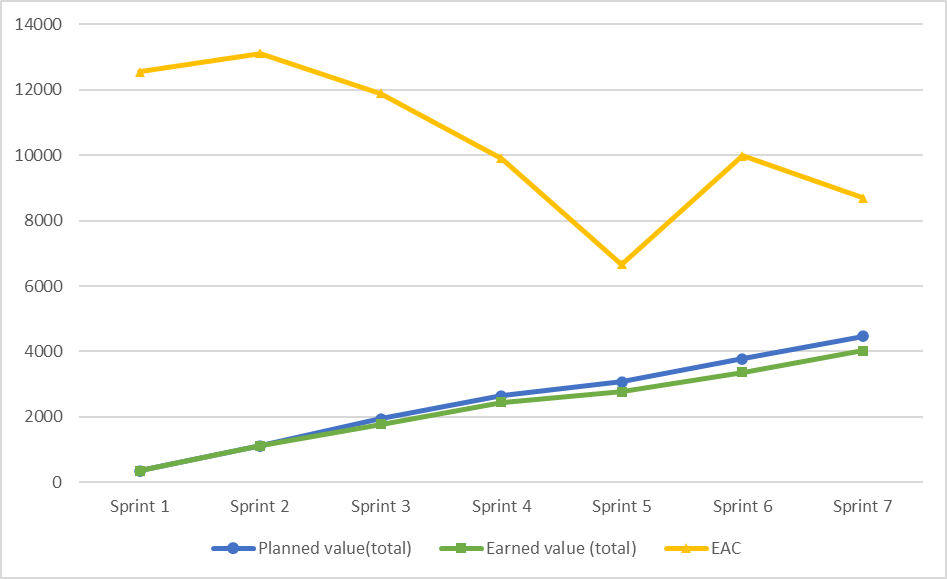
\includegraphics[width=\linewidth]{pdq/planned_earned-RTB.png}
    \caption{Planned Value e Earned Value totali}
    \label{fig:Grafico MPC02 e MPC04}
\end{figure}
Il grafico mostra che Earned Value e Planned Value rientrano nei rispettivi intervalli accettabili, quindi nel futuro si mirerà a portare entrambe a coincidere per raggiungere il valore ottimo.

\subsection{MPC03: Actual Cost, MPC07 Estimate at Completion e MPC08: Estimate to Complete}
\begin{figure}[H]
    \centering
    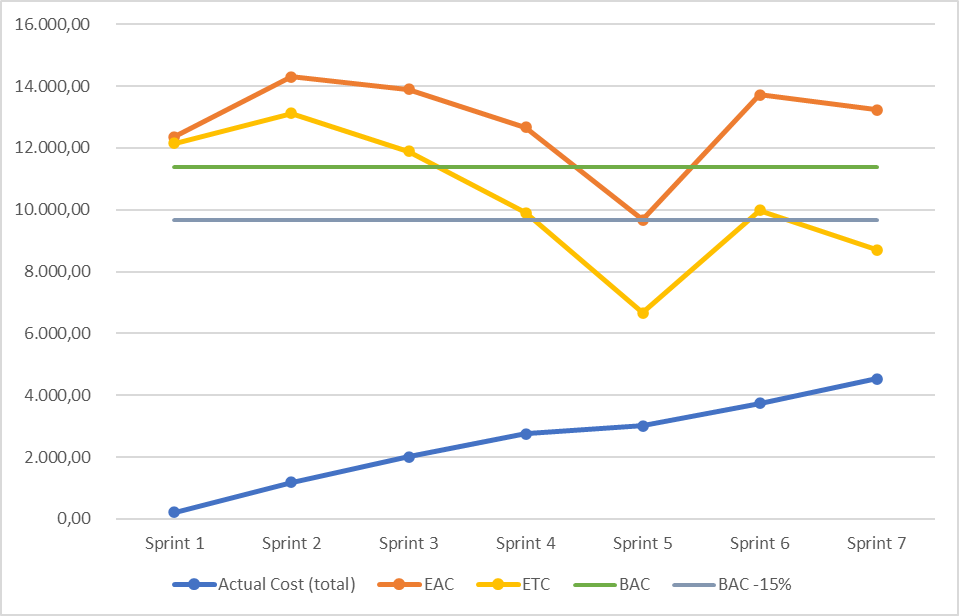
\includegraphics[width=\linewidth]{pdq/EAC_ETC-RTB.png}
    \caption{Actual Cost, Estimate at Completion e Estimate to Complete}
    \label{fig:Grafico MPC03, MPC07 e MPC08}
\end{figure}
Il grafico mostra che l'Estimate at Completion è principalmente oltre il valore accettabile del Budget at Completion, ad eccezione per lo \term{Sprint} 5. La differenza in quest'ultimo è dovuta alle condizioni causate dalla sessione di esami che hanno portato a notevole differenza tra le ore stimate e le ore effettivamente impiegate durante lo \term{Sprint}.\\
L'Estimate to Complete mostra un trend positivo tra lo \term{Sprint} 6 e 7 che si riflette positivamente sull'Estimate at Completion; sarà quindi necessario prendere misure atte a mantenere tale trend, in modo da riportare l'EAC dentro l'intervallo accettabile.

\subsection{MPC06: Schedule Performance Index}
\begin{figure}[H]
    \centering
    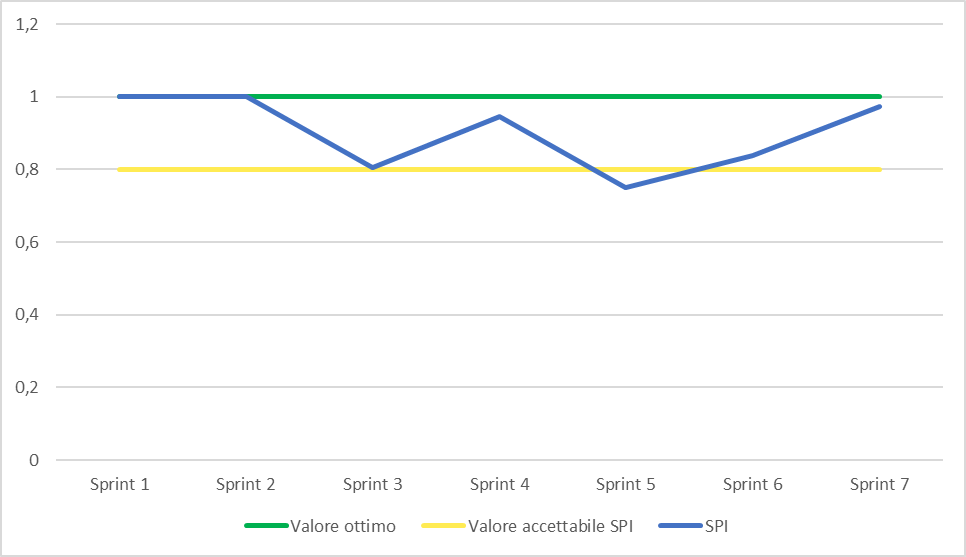
\includegraphics[width=\linewidth]{pdq/SPI-RTB.png}
    \caption{Schedule Performance Index}
    \label{fig:Grafico MPC06}
\end{figure}
Il grafico mostra che nonostante le fluttuazioni, lo Schedule Performance Index è rimasto prevalentemente nel range accettabile. Unica eccezione il valore durante lo \term{Sprint} 5 in cui è sceso sotto la soglia accettabile, per poi recuperare negli \term{Sprint} successivi e quindi plausibilmente causato dalla coincidenza con la sessione di esami universitari.

\subsection{MPC05: Cost Performance Index}
\begin{figure}[H]
    \centering
    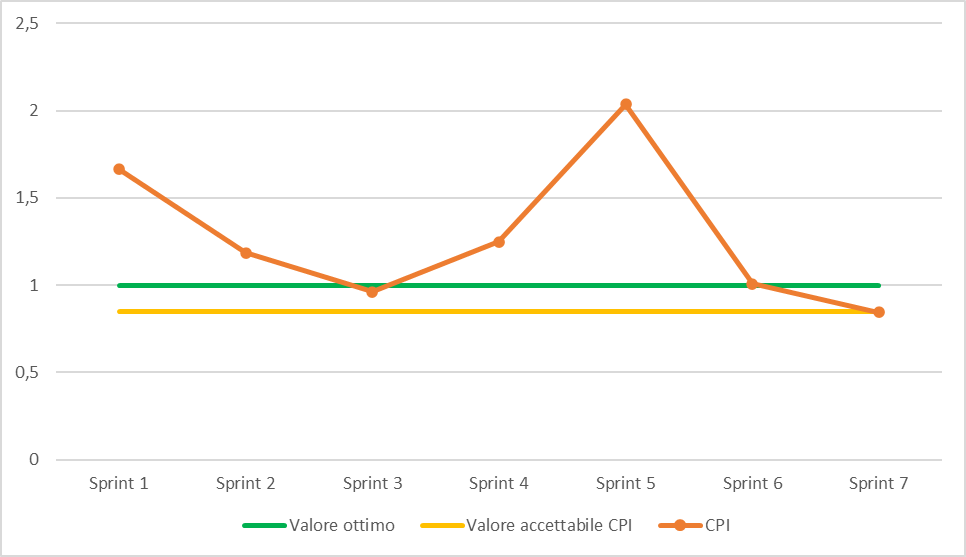
\includegraphics[width=\linewidth]{pdq/CPI-RTB.png}
    \caption{Cost Performance Index}
    \label{fig:Grafico MPC05}
\end{figure}
Il grafico mostra che l'indice Cost Performance Index ha prevalentemente avuto valori inferiori alla soglia minima accettabile, ad eccezione degli \term{Sprint} 1, 4 e 5 che sono entro o oltre l'intervallo accettabile.\\
I valori negli \term{Sprint} 6 e 7, nonostante la non sufficienza, mostrano un trend positivo dell'indice che sarà necessario mantenere nelle fasi successive per fare in modo che rientri nella zona accettabile.

\subsection{MPC10: Indice di Gulpease}
\begin{figure}[H]
    \centering
    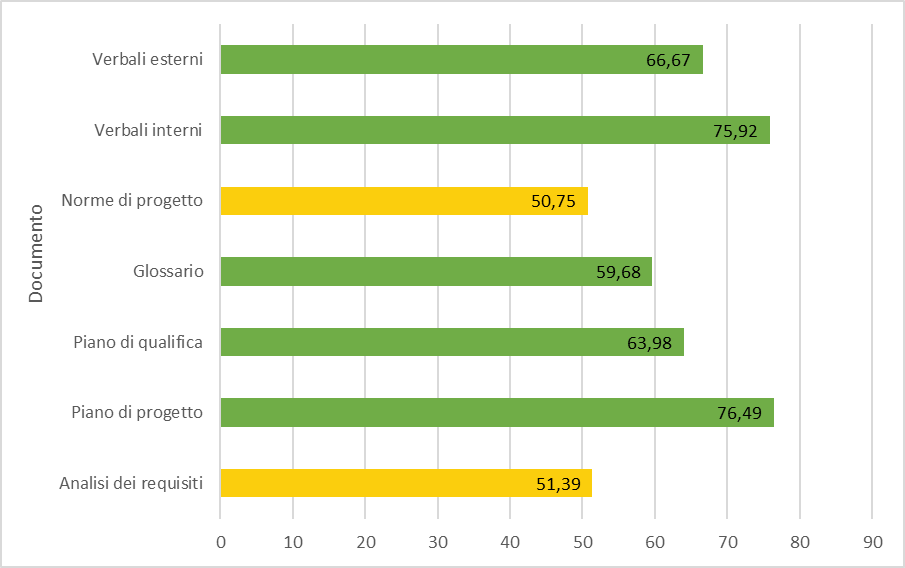
\includegraphics[width=\linewidth]{pdq/Gulpease-RTB.png}
    \caption{Indice di Gulpease}
    \label{fig:Grafico MPC10}
\end{figure}
Il grafico mostra che il valore dell'Indice di Gulpease della documentazione prodotta risulta sempre superiore alla soglia del valore accettabile, con la maggior parte della documentazione oltre la soglia ottima.\\
Le Norme di Progetto e l'\term{Analisi dei requisiti} sono i documenti con l'indice più basso, ma va segnalato che anche il Glossario (59,68) sfiora appena la soglia ottima, senza tuttavia superarla. Poiché si tratta di documenti tecnici, la presenza di terminologia specifica e frasi articolate può abbassare marginalmente questo indice senza comprometterne la reale leggibilità per gli addetti ai lavori. Pertanto, un intervento correttivo mirato unicamente all'innalzamento dell'indice non è ritenuto prioritario, ma se in futuro si renderanno necessarie modifiche a questi documenti, si presterà attenzione a semplificarne la struttura linguistica.

\end{document}